\documentclass[1p]{elsarticle_modified}
%\bibliographystyle{elsarticle-num}

%\usepackage[colorlinks]{hyperref}
%\usepackage{abbrmath_seonhwa} %\Abb, \Ascr, \Acal ,\Abf, \Afrak
\usepackage{amsfonts}
\usepackage{amssymb}
\usepackage{amsmath}
\usepackage{amsthm}
\usepackage{scalefnt}
\usepackage{amsbsy}
\usepackage{kotex}
\usepackage{caption}
\usepackage{subfig}
\usepackage{color}
\usepackage{graphicx}
\usepackage{xcolor} %% white, black, red, green, blue, cyan, magenta, yellow
\usepackage{float}
\usepackage{setspace}
\usepackage{hyperref}

\usepackage{tikz}
\usetikzlibrary{arrows}

\usepackage{multirow}
\usepackage{array} % fixed length table
\usepackage{hhline}

%%%%%%%%%%%%%%%%%%%%%
\makeatletter
\renewcommand*\env@matrix[1][\arraystretch]{%
	\edef\arraystretch{#1}%
	\hskip -\arraycolsep
	\let\@ifnextchar\new@ifnextchar
	\array{*\c@MaxMatrixCols c}}
\makeatother %https://tex.stackexchange.com/questions/14071/how-can-i-increase-the-line-spacing-in-a-matrix
%%%%%%%%%%%%%%%

\usepackage[normalem]{ulem}

\newcommand{\msout}[1]{\ifmmode\text{\sout{\ensuremath{#1}}}\else\sout{#1}\fi}
%SOURCE: \msout is \stkout macro in https://tex.stackexchange.com/questions/20609/strikeout-in-math-mode

\newcommand{\cancel}[1]{
	\ifmmode
	{\color{red}\msout{#1}}
	\else
	{\color{red}\sout{#1}}
	\fi
}

\newcommand{\add}[1]{
	{\color{blue}\uwave{#1}}
}

\newcommand{\replace}[2]{
	\ifmmode
	{\color{red}\msout{#1}}{\color{blue}\uwave{#2}}
	\else
	{\color{red}\sout{#1}}{\color{blue}\uwave{#2}}
	\fi
}

\newcommand{\Sol}{\mathcal{S}} %segment
\newcommand{\D}{D} %diagram
\newcommand{\A}{\mathcal{A}} %arc


%%%%%%%%%%%%%%%%%%%%%%%%%%%%%5 test

\def\sl{\operatorname{\textup{SL}}(2,\Cbb)}
\def\psl{\operatorname{\textup{PSL}}(2,\Cbb)}
\def\quan{\mkern 1mu \triangleright \mkern 1mu}

\theoremstyle{definition}
\newtheorem{thm}{Theorem}[section]
\newtheorem{prop}[thm]{Proposition}
\newtheorem{lem}[thm]{Lemma}
\newtheorem{ques}[thm]{Question}
\newtheorem{cor}[thm]{Corollary}
\newtheorem{defn}[thm]{Definition}
\newtheorem{exam}[thm]{Example}
\newtheorem{rmk}[thm]{Remark}
\newtheorem{alg}[thm]{Algorithm}

\newcommand{\I}{\sqrt{-1}}
\begin{document}

%\begin{frontmatter}
%
%\title{Boundary parabolic representations of knots up to 8 crossings}
%
%%% Group authors per affiliation:
%\author{Yunhi Cho} 
%\address{Department of Mathematics, University of Seoul, Seoul, Korea}
%\ead{yhcho@uos.ac.kr}
%
%
%\author{Seonhwa Kim} %\fnref{s_kim}}
%\address{Center for Geometry and Physics, Institute for Basic Science, Pohang, 37673, Korea}
%\ead{ryeona17@ibs.re.kr}
%
%\author{Hyuk Kim}
%\address{Department of Mathematical Sciences, Seoul National University, Seoul 08826, Korea}
%\ead{hyukkim@snu.ac.kr}
%
%\author{Seokbeom Yoon}
%\address{Department of Mathematical Sciences, Seoul National University, Seoul, 08826,  Korea}
%\ead{sbyoon15@snu.ac.kr}
%
%\begin{abstract}
%We find all boundary parabolic representation of knots up to 8 crossings.
%
%\end{abstract}
%\begin{keyword}
%    \MSC[2010] 57M25 
%\end{keyword}
%
%\end{frontmatter}

%\linenumbers
%\tableofcontents
%
\newcommand\colored[1]{\textcolor{white}{\rule[-0.35ex]{0.8em}{1.4ex}}\kern-0.8em\color{red} #1}%
%\newcommand\colored[1]{\textcolor{white}{ #1}\kern-2.17ex	\textcolor{white}{ #1}\kern-1.81ex	\textcolor{white}{ #1}\kern-2.15ex\color{red}#1	}

{\Large $\underline{12a_{0778}~(K12a_{0778})}$}

\setlength{\tabcolsep}{10pt}
\renewcommand{\arraystretch}{1.6}
\vspace{1cm}\begin{tabular}{m{100pt}>{\centering\arraybackslash}m{274pt}}
\multirow{5}{120pt}{
	\centering
	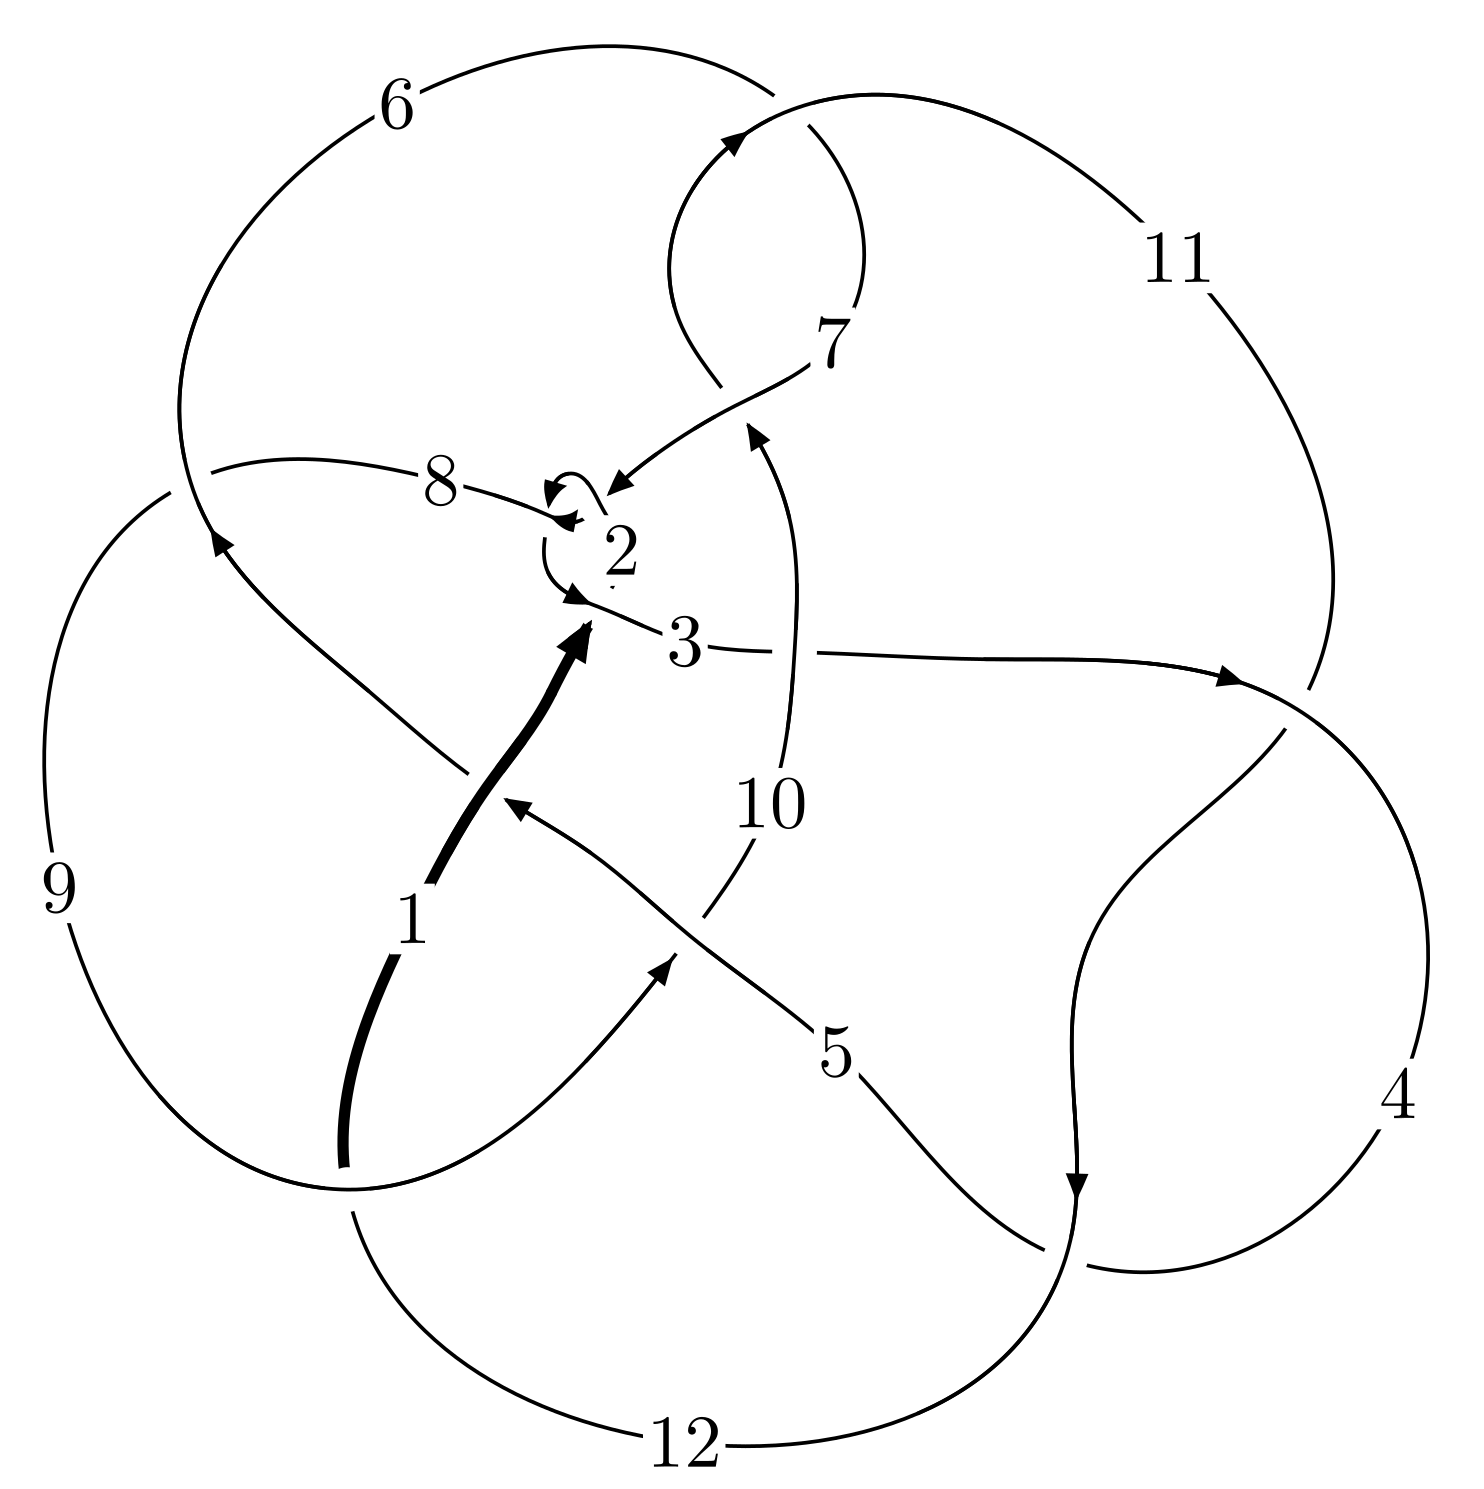
\includegraphics[width=112pt]{../../../GIT/diagram.site/Diagrams/png/1579_12a_0778.png}\\
\ \ \ A knot diagram\footnotemark}&
\allowdisplaybreaks
\textbf{Linearized knot diagam} \\
\cline{2-2}
 &
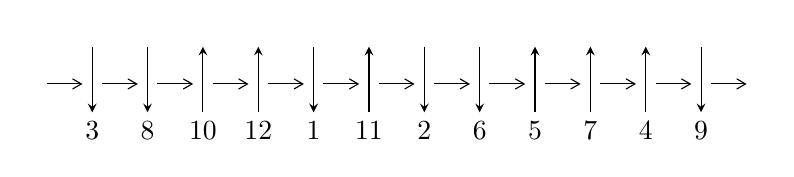
\begin{tikzpicture}[x=20pt, y=17pt]
	% nodes
	\node (C0) at (0, 0) {};
	\node (C1) at (1, 0) {};
	\node (C1U) at (1, +1) {};
	\node (C1D) at (1, -1) {3};

	\node (C2) at (2, 0) {};
	\node (C2U) at (2, +1) {};
	\node (C2D) at (2, -1) {8};

	\node (C3) at (3, 0) {};
	\node (C3U) at (3, +1) {};
	\node (C3D) at (3, -1) {10};

	\node (C4) at (4, 0) {};
	\node (C4U) at (4, +1) {};
	\node (C4D) at (4, -1) {12};

	\node (C5) at (5, 0) {};
	\node (C5U) at (5, +1) {};
	\node (C5D) at (5, -1) {1};

	\node (C6) at (6, 0) {};
	\node (C6U) at (6, +1) {};
	\node (C6D) at (6, -1) {11};

	\node (C7) at (7, 0) {};
	\node (C7U) at (7, +1) {};
	\node (C7D) at (7, -1) {2};

	\node (C8) at (8, 0) {};
	\node (C8U) at (8, +1) {};
	\node (C8D) at (8, -1) {6};

	\node (C9) at (9, 0) {};
	\node (C9U) at (9, +1) {};
	\node (C9D) at (9, -1) {5};

	\node (C10) at (10, 0) {};
	\node (C10U) at (10, +1) {};
	\node (C10D) at (10, -1) {7};

	\node (C11) at (11, 0) {};
	\node (C11U) at (11, +1) {};
	\node (C11D) at (11, -1) {4};

	\node (C12) at (12, 0) {};
	\node (C12U) at (12, +1) {};
	\node (C12D) at (12, -1) {9};
	\node (C13) at (13, 0) {};

	% arrows
	\draw[->,>={angle 60}]
	(C0) edge (C1) (C1) edge (C2) (C2) edge (C3) (C3) edge (C4) (C4) edge (C5) (C5) edge (C6) (C6) edge (C7) (C7) edge (C8) (C8) edge (C9) (C9) edge (C10) (C10) edge (C11) (C11) edge (C12) (C12) edge (C13) ;	\draw[->,>=stealth]
	(C1U) edge (C1D) (C2U) edge (C2D) (C3D) edge (C3U) (C4D) edge (C4U) (C5U) edge (C5D) (C6D) edge (C6U) (C7U) edge (C7D) (C8U) edge (C8D) (C9D) edge (C9U) (C10D) edge (C10U) (C11D) edge (C11U) (C12U) edge (C12D) ;
	\end{tikzpicture} \\
\hhline{~~} \\& 
\textbf{Solving Sequence} \\ \cline{2-2} 
 &
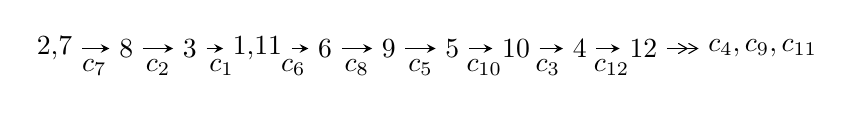
\begin{tikzpicture}[x=23pt, y=7pt]
	% node
	\node (A0) at (-1/8, 0) {2,7};
	\node (A1) at (1, 0) {8};
	\node (A2) at (2, 0) {3};
	\node (A3) at (49/16, 0) {1,11};
	\node (A4) at (33/8, 0) {6};
	\node (A5) at (41/8, 0) {9};
	\node (A6) at (49/8, 0) {5};
	\node (A7) at (57/8, 0) {10};
	\node (A8) at (65/8, 0) {4};
	\node (A9) at (73/8, 0) {12};
	\node (C1) at (1/2, -1) {$c_{7}$};
	\node (C2) at (3/2, -1) {$c_{2}$};
	\node (C3) at (5/2, -1) {$c_{1}$};
	\node (C4) at (29/8, -1) {$c_{6}$};
	\node (C5) at (37/8, -1) {$c_{8}$};
	\node (C6) at (45/8, -1) {$c_{5}$};
	\node (C7) at (53/8, -1) {$c_{10}$};
	\node (C8) at (61/8, -1) {$c_{3}$};
	\node (C9) at (69/8, -1) {$c_{12}$};
	\node (A10) at (11, 0) {$c_{4},c_{9},c_{11}$};

	% edge
	\draw[->,>=stealth]	
	(A0) edge (A1) (A1) edge (A2) (A2) edge (A3) (A3) edge (A4) (A4) edge (A5) (A5) edge (A6) (A6) edge (A7) (A7) edge (A8) (A8) edge (A9) ;
	\draw[->>,>={angle 60}]	
	(A9) edge (A10);
\end{tikzpicture} \\ 

\end{tabular} \\

\footnotetext{
The image of knot diagram is generated by the software ``\textbf{Draw programme}" developed by Andrew Bartholomew(\url{http://www.layer8.co.uk/maths/draw/index.htm\#Running-draw}), where we modified some parts for our purpose(\url{https://github.com/CATsTAILs/LinksPainter}).
}\phantom \\ \newline 
\centering \textbf{Ideals for irreducible components\footnotemark of $X_{\text{par}}$} 
 
\begin{align*}
I^u_{1}&=\langle 
2.83192\times10^{557} u^{177}-6.25443\times10^{556} u^{176}+\cdots+5.07791\times10^{558} b-2.49182\times10^{560},\\
\phantom{I^u_{1}}&\phantom{= \langle  }1.66942\times10^{562} u^{177}+4.31753\times10^{560} u^{176}+\cdots+5.53848\times10^{562} a-9.73150\times10^{564},\\
\phantom{I^u_{1}}&\phantom{= \langle  }u^{178}- u^{177}+\cdots-3043 u+839\rangle \\
I^u_{2}&=\langle 
-8317077395 u^{45}-6692694951 u^{44}+\cdots+1782959561 b-14602686346,\\
\phantom{I^u_{2}}&\phantom{= \langle  }-39738567974 u^{45}-7168731592677 u^{44}+\cdots+622252886789 a+2806256180785,\\
\phantom{I^u_{2}}&\phantom{= \langle  }u^{46}-13 u^{44}+\cdots+3 u+1\rangle \\
\\
\end{align*}
\raggedright * 2 irreducible components of $\dim_{\mathbb{C}}=0$, with total 224 representations.\\
\footnotetext{All coefficients of polynomials are rational numbers. But the coefficients are sometimes approximated in decimal forms when there is not enough margin.}
\newpage
\renewcommand{\arraystretch}{1}
\centering \section*{I. $I^u_{1}= \langle 2.83\times10^{557} u^{177}-6.25\times10^{556} u^{176}+\cdots+5.08\times10^{558} b-2.49\times10^{560},\;1.67\times10^{562} u^{177}+4.32\times10^{560} u^{176}+\cdots+5.54\times10^{562} a-9.73\times10^{564},\;u^{178}- u^{177}+\cdots-3043 u+839 \rangle$}
\flushleft \textbf{(i) Arc colorings}\\
\begin{tabular}{m{7pt} m{180pt} m{7pt} m{180pt} }
\flushright $a_{2}=$&$\begin{pmatrix}0\\u\end{pmatrix}$ \\
\flushright $a_{7}=$&$\begin{pmatrix}1\\0\end{pmatrix}$ \\
\flushright $a_{8}=$&$\begin{pmatrix}1\\u^2\end{pmatrix}$ \\
\flushright $a_{3}=$&$\begin{pmatrix}- u\\- u^3+u\end{pmatrix}$ \\
\flushright $a_{1}=$&$\begin{pmatrix}u^3\\u^5- u^3+u\end{pmatrix}$ \\
\flushright $a_{11}=$&$\begin{pmatrix}-0.301422 u^{177}-0.00779552 u^{176}+\cdots-467.541 u+175.707\\-0.0557695 u^{177}+0.0123169 u^{176}+\cdots-99.9826 u+49.0718\end{pmatrix}$ \\
\flushright $a_{6}=$&$\begin{pmatrix}-0.148718 u^{177}+0.164496 u^{176}+\cdots+198.358 u-54.6244\\-0.0620492 u^{177}+0.137246 u^{176}+\cdots+315.427 u-72.3130\end{pmatrix}$ \\
\flushright $a_{9}=$&$\begin{pmatrix}-0.343320 u^{177}-0.0126359 u^{176}+\cdots-811.691 u+297.191\\0.0116331 u^{177}-0.0316594 u^{176}+\cdots-105.316 u+43.9533\end{pmatrix}$ \\
\flushright $a_{5}=$&$\begin{pmatrix}-0.117881 u^{177}+0.0434351 u^{176}+\cdots+15.4920 u-18.5703\\-0.0604457 u^{177}+0.0849581 u^{176}+\cdots+172.096 u-31.1648\end{pmatrix}$ \\
\flushright $a_{10}=$&$\begin{pmatrix}-0.245653 u^{177}-0.0201125 u^{176}+\cdots-367.558 u+126.635\\-0.0557695 u^{177}+0.0123169 u^{176}+\cdots-99.9826 u+49.0718\end{pmatrix}$ \\
\flushright $a_{4}=$&$\begin{pmatrix}0.0646156 u^{177}-0.244183 u^{176}+\cdots+260.057 u-165.861\\0.0305702 u^{177}-0.0849381 u^{176}+\cdots-118.034 u+3.73802\end{pmatrix}$ \\
\flushright $a_{12}=$&$\begin{pmatrix}0.120327 u^{177}+0.117052 u^{176}+\cdots+179.284 u-10.9664\\-0.113303 u^{177}+0.0278594 u^{176}+\cdots-245.370 u+99.0238\end{pmatrix}$\\&\end{tabular}
\flushleft \textbf{(ii) Obstruction class $= -1$}\\~\\
\flushleft \textbf{(iii) Cusp Shapes $= -0.0572173 u^{177}+0.0141848 u^{176}+\cdots-447.259 u+188.065$}\\~\\
\newpage\renewcommand{\arraystretch}{1}
\flushleft \textbf{(iv) u-Polynomials at the component}\newline \\
\begin{tabular}{m{50pt}|m{274pt}}
Crossings & \hspace{64pt}u-Polynomials at each crossing \\
\hline $$\begin{aligned}c_{1}\end{aligned}$$&$\begin{aligned}
&u^{178}+85 u^{177}+\cdots+12261791 u+703921
\end{aligned}$\\
\hline $$\begin{aligned}c_{2},c_{7}\end{aligned}$$&$\begin{aligned}
&u^{178}+u^{177}+\cdots+3043 u+839
\end{aligned}$\\
\hline $$\begin{aligned}c_{3}\end{aligned}$$&$\begin{aligned}
&u^{178}+u^{177}+\cdots+354196 u+339257
\end{aligned}$\\
\hline $$\begin{aligned}c_{4},c_{11}\end{aligned}$$&$\begin{aligned}
&u^{178}+u^{177}+\cdots-563010 u+122123
\end{aligned}$\\
\hline $$\begin{aligned}c_{5}\end{aligned}$$&$\begin{aligned}
&u^{178}+5 u^{177}+\cdots+300 u+179
\end{aligned}$\\
\hline $$\begin{aligned}c_{6},c_{10}\end{aligned}$$&$\begin{aligned}
&u^{178}+46 u^{176}+\cdots+147913 u+12577
\end{aligned}$\\
\hline $$\begin{aligned}c_{8}\end{aligned}$$&$\begin{aligned}
&u^{178}-8 u^{177}+\cdots-193237632 u+17520832
\end{aligned}$\\
\hline $$\begin{aligned}c_{9}\end{aligned}$$&$\begin{aligned}
&u^{178}-3 u^{177}+\cdots-316 u+83
\end{aligned}$\\
\hline $$\begin{aligned}c_{12}\end{aligned}$$&$\begin{aligned}
&u^{178}+6 u^{177}+\cdots-2444512 u+375469
\end{aligned}$\\
\hline
\end{tabular}\\~\\
\newpage\renewcommand{\arraystretch}{1}
\flushleft \textbf{(v) Riley Polynomials at the component}\newline \\
\begin{tabular}{m{50pt}|m{274pt}}
Crossings & \hspace{64pt}Riley Polynomials at each crossing \\
\hline $$\begin{aligned}c_{1}\end{aligned}$$&$\begin{aligned}
&y^{178}+31 y^{177}+\cdots-583680219959 y+495504774241
\end{aligned}$\\
\hline $$\begin{aligned}c_{2},c_{7}\end{aligned}$$&$\begin{aligned}
&y^{178}-85 y^{177}+\cdots-12261791 y+703921
\end{aligned}$\\
\hline $$\begin{aligned}c_{3}\end{aligned}$$&$\begin{aligned}
&y^{178}-5 y^{177}+\cdots+10288606046288 y+115095312049
\end{aligned}$\\
\hline $$\begin{aligned}c_{4},c_{11}\end{aligned}$$&$\begin{aligned}
&y^{178}-133 y^{177}+\cdots-108608624088 y+14914027129
\end{aligned}$\\
\hline $$\begin{aligned}c_{5}\end{aligned}$$&$\begin{aligned}
&y^{178}-19 y^{177}+\cdots+637456 y+32041
\end{aligned}$\\
\hline $$\begin{aligned}c_{6},c_{10}\end{aligned}$$&$\begin{aligned}
&y^{178}+92 y^{177}+\cdots+9058774801 y+158180929
\end{aligned}$\\
\hline $$\begin{aligned}c_{8}\end{aligned}$$&$\begin{aligned}
&y^{178}+8 y^{177}+\cdots+24453354177839104 y+306979553972224
\end{aligned}$\\
\hline $$\begin{aligned}c_{9}\end{aligned}$$&$\begin{aligned}
&y^{178}-35 y^{177}+\cdots-612962 y+6889
\end{aligned}$\\
\hline $$\begin{aligned}c_{12}\end{aligned}$$&$\begin{aligned}
&y^{178}+40 y^{177}+\cdots+11873515289866 y+140976969961
\end{aligned}$\\
\hline
\end{tabular}\\~\\
\newpage\flushleft \textbf{(vi) Complex Volumes and Cusp Shapes}
$$\begin{array}{c|c|c}  
\text{Solutions to }I^u_{1}& \I (\text{vol} + \sqrt{-1}CS) & \text{Cusp shape}\\
 \hline 
\begin{aligned}
u &= \phantom{-}1.002900 + 0.076332 I \\
a &= \phantom{-}0.410643 - 0.082087 I \\
b &= \phantom{-}0.579253 + 0.123214 I\end{aligned}
 & -2.11950 - 0.08413 I & \phantom{-0.000000 } 0 \\ \hline\begin{aligned}
u &= \phantom{-}1.002900 - 0.076332 I \\
a &= \phantom{-}0.410643 + 0.082087 I \\
b &= \phantom{-}0.579253 - 0.123214 I\end{aligned}
 & -2.11950 + 0.08413 I & \phantom{-0.000000 } 0 \\ \hline\begin{aligned}
u &= -0.226401 + 0.966400 I \\
a &= \phantom{-}0.409044 + 0.569674 I \\
b &= -0.439674 + 0.950963 I\end{aligned}
 & -0.53209 - 2.15422 I & \phantom{-0.000000 } 0 \\ \hline\begin{aligned}
u &= -0.226401 - 0.966400 I \\
a &= \phantom{-}0.409044 - 0.569674 I \\
b &= -0.439674 - 0.950963 I\end{aligned}
 & -0.53209 + 2.15422 I & \phantom{-0.000000 } 0 \\ \hline\begin{aligned}
u &= -0.335859 + 0.954059 I \\
a &= -0.159374 - 0.553582 I \\
b &= \phantom{-}0.536749 - 1.176660 I\end{aligned}
 & -1.52044 - 8.62842 I & \phantom{-0.000000 } 0 \\ \hline\begin{aligned}
u &= -0.335859 - 0.954059 I \\
a &= -0.159374 + 0.553582 I \\
b &= \phantom{-}0.536749 + 1.176660 I\end{aligned}
 & -1.52044 + 8.62842 I & \phantom{-0.000000 } 0 \\ \hline\begin{aligned}
u &= \phantom{-}0.919829 + 0.360834 I \\
a &= \phantom{-}3.14733 + 2.88557 I \\
b &= -0.080521 + 0.756472 I\end{aligned}
 & \phantom{-}1.56137 + 3.49668 I & \phantom{-0.000000 } 0 \\ \hline\begin{aligned}
u &= \phantom{-}0.919829 - 0.360834 I \\
a &= \phantom{-}3.14733 - 2.88557 I \\
b &= -0.080521 - 0.756472 I\end{aligned}
 & \phantom{-}1.56137 - 3.49668 I & \phantom{-0.000000 } 0 \\ \hline\begin{aligned}
u &= \phantom{-}0.374555 + 0.943169 I \\
a &= -0.356602 + 0.476093 I \\
b &= \phantom{-}0.677133 + 1.219760 I\end{aligned}
 & \phantom{-}3.2314 + 14.8369 I & \phantom{-0.000000 } 0 \\ \hline\begin{aligned}
u &= \phantom{-}0.374555 - 0.943169 I \\
a &= -0.356602 - 0.476093 I \\
b &= \phantom{-}0.677133 - 1.219760 I\end{aligned}
 & \phantom{-}3.2314 - 14.8369 I & \phantom{-0.000000 } 0\\
 \hline 
 \end{array}$$\newpage$$\begin{array}{c|c|c}  
\text{Solutions to }I^u_{1}& \I (\text{vol} + \sqrt{-1}CS) & \text{Cusp shape}\\
 \hline 
\begin{aligned}
u &= -0.733219 + 0.657144 I \\
a &= \phantom{-}0.290021 - 0.279870 I \\
b &= -0.720709 - 0.133801 I\end{aligned}
 & \phantom{-}2.84448 + 0.62683 I & \phantom{-0.000000 } 0 \\ \hline\begin{aligned}
u &= -0.733219 - 0.657144 I \\
a &= \phantom{-}0.290021 + 0.279870 I \\
b &= -0.720709 + 0.133801 I\end{aligned}
 & \phantom{-}2.84448 - 0.62683 I & \phantom{-0.000000 } 0 \\ \hline\begin{aligned}
u &= \phantom{-}0.879338 + 0.433465 I \\
a &= \phantom{-}0.674827 - 0.733572 I \\
b &= -0.627845 - 0.975355 I\end{aligned}
 & \phantom{-}2.79221 + 0.32953 I & \phantom{-0.000000 } 0 \\ \hline\begin{aligned}
u &= \phantom{-}0.879338 - 0.433465 I \\
a &= \phantom{-}0.674827 + 0.733572 I \\
b &= -0.627845 + 0.975355 I\end{aligned}
 & \phantom{-}2.79221 - 0.32953 I & \phantom{-0.000000 } 0 \\ \hline\begin{aligned}
u &= \phantom{-}0.925580 + 0.310759 I \\
a &= -1.67998 - 1.78962 I \\
b &= \phantom{-}0.121356 + 0.308713 I\end{aligned}
 & \phantom{-}1.66529 - 6.27208 I & \phantom{-0.000000 } 0 \\ \hline\begin{aligned}
u &= \phantom{-}0.925580 - 0.310759 I \\
a &= -1.67998 + 1.78962 I \\
b &= \phantom{-}0.121356 - 0.308713 I\end{aligned}
 & \phantom{-}1.66529 + 6.27208 I & \phantom{-0.000000 } 0 \\ \hline\begin{aligned}
u &= -0.997517 + 0.261432 I \\
a &= -0.648349 + 0.344258 I \\
b &= \phantom{-}0.289800 - 0.362909 I\end{aligned}
 & -3.41325 + 3.33568 I & \phantom{-0.000000 } 0 \\ \hline\begin{aligned}
u &= -0.997517 - 0.261432 I \\
a &= -0.648349 - 0.344258 I \\
b &= \phantom{-}0.289800 + 0.362909 I\end{aligned}
 & -3.41325 - 3.33568 I & \phantom{-0.000000 } 0 \\ \hline\begin{aligned}
u &= -0.503693 + 0.823683 I \\
a &= -0.0536241 - 0.0652593 I \\
b &= \phantom{-}0.694699 - 1.139340 I\end{aligned}
 & \phantom{-}4.22856 - 6.39408 I & \phantom{-0.000000 } 0 \\ \hline\begin{aligned}
u &= -0.503693 - 0.823683 I \\
a &= -0.0536241 + 0.0652593 I \\
b &= \phantom{-}0.694699 + 1.139340 I\end{aligned}
 & \phantom{-}4.22856 + 6.39408 I & \phantom{-0.000000 } 0\\
 \hline 
 \end{array}$$\newpage$$\begin{array}{c|c|c}  
\text{Solutions to }I^u_{1}& \I (\text{vol} + \sqrt{-1}CS) & \text{Cusp shape}\\
 \hline 
\begin{aligned}
u &= \phantom{-}0.863451 + 0.430814 I \\
a &= -1.35124 - 3.01221 I \\
b &= \phantom{-}0.421417 - 1.034660 I\end{aligned}
 & \phantom{-}2.84586 - 3.91339 I & \phantom{-0.000000 } 0 \\ \hline\begin{aligned}
u &= \phantom{-}0.863451 - 0.430814 I \\
a &= -1.35124 + 3.01221 I \\
b &= \phantom{-}0.421417 + 1.034660 I\end{aligned}
 & \phantom{-}2.84586 + 3.91339 I & \phantom{-0.000000 } 0 \\ \hline\begin{aligned}
u &= -0.932656 + 0.220528 I \\
a &= -0.026254 - 0.622186 I \\
b &= -0.752555 + 0.549421 I\end{aligned}
 & -3.02952 - 2.41652 I & \phantom{-0.000000 } 0 \\ \hline\begin{aligned}
u &= -0.932656 - 0.220528 I \\
a &= -0.026254 + 0.622186 I \\
b &= -0.752555 - 0.549421 I\end{aligned}
 & -3.02952 + 2.41652 I & \phantom{-0.000000 } 0 \\ \hline\begin{aligned}
u &= -0.961071 + 0.420548 I \\
a &= \phantom{-}0.69112 + 1.38885 I \\
b &= \phantom{-}1.43328 + 0.01277 I\end{aligned}
 & \phantom{-}3.29043 + 3.04918 I & \phantom{-0.000000 } 0 \\ \hline\begin{aligned}
u &= -0.961071 - 0.420548 I \\
a &= \phantom{-}0.69112 - 1.38885 I \\
b &= \phantom{-}1.43328 - 0.01277 I\end{aligned}
 & \phantom{-}3.29043 - 3.04918 I & \phantom{-0.000000 } 0 \\ \hline\begin{aligned}
u &= -0.791467 + 0.690929 I \\
a &= \phantom{-}0.642459 + 0.639450 I \\
b &= \phantom{-}0.357063 - 0.611371 I\end{aligned}
 & \phantom{-}4.26263 + 0.47129 I & \phantom{-0.000000 } 0 \\ \hline\begin{aligned}
u &= -0.791467 - 0.690929 I \\
a &= \phantom{-}0.642459 - 0.639450 I \\
b &= \phantom{-}0.357063 + 0.611371 I\end{aligned}
 & \phantom{-}4.26263 - 0.47129 I & \phantom{-0.000000 } 0 \\ \hline\begin{aligned}
u &= -0.860791 + 0.400076 I \\
a &= -0.033598 - 1.094830 I \\
b &= -1.348070 - 0.150928 I\end{aligned}
 & \phantom{-}3.71483 + 0.26000 I & \phantom{-0.000000 } 0 \\ \hline\begin{aligned}
u &= -0.860791 - 0.400076 I \\
a &= -0.033598 + 1.094830 I \\
b &= -1.348070 + 0.150928 I\end{aligned}
 & \phantom{-}3.71483 - 0.26000 I & \phantom{-0.000000 } 0\\
 \hline 
 \end{array}$$\newpage$$\begin{array}{c|c|c}  
\text{Solutions to }I^u_{1}& \I (\text{vol} + \sqrt{-1}CS) & \text{Cusp shape}\\
 \hline 
\begin{aligned}
u &= \phantom{-}0.455344 + 0.832194 I \\
a &= \phantom{-}0.102653 + 0.514193 I \\
b &= \phantom{-}0.418681 + 0.944244 I\end{aligned}
 & \phantom{-}0.802586 - 0.654897 I & \phantom{-0.000000 } 0 \\ \hline\begin{aligned}
u &= \phantom{-}0.455344 - 0.832194 I \\
a &= \phantom{-}0.102653 - 0.514193 I \\
b &= \phantom{-}0.418681 - 0.944244 I\end{aligned}
 & \phantom{-}0.802586 + 0.654897 I & \phantom{-0.000000 } 0 \\ \hline\begin{aligned}
u &= \phantom{-}1.000000 + 0.351874 I \\
a &= \phantom{-}0.74966 + 2.66662 I \\
b &= \phantom{-}0.33424 + 1.39910 I\end{aligned}
 & -3.13518 + 3.47455 I & \phantom{-0.000000 } 0 \\ \hline\begin{aligned}
u &= \phantom{-}1.000000 - 0.351874 I \\
a &= \phantom{-}0.74966 - 2.66662 I \\
b &= \phantom{-}0.33424 - 1.39910 I\end{aligned}
 & -3.13518 - 3.47455 I & \phantom{-0.000000 } 0 \\ \hline\begin{aligned}
u &= -0.537889 + 0.769907 I \\
a &= -0.343867 - 0.772663 I \\
b &= \phantom{-}0.639669 - 0.652252 I\end{aligned}
 & \phantom{-}6.38925 + 5.50798 I & \phantom{-0.000000 } 0 \\ \hline\begin{aligned}
u &= -0.537889 - 0.769907 I \\
a &= -0.343867 + 0.772663 I \\
b &= \phantom{-}0.639669 + 0.652252 I\end{aligned}
 & \phantom{-}6.38925 - 5.50798 I & \phantom{-0.000000 } 0 \\ \hline\begin{aligned}
u &= -0.534702 + 0.760598 I \\
a &= \phantom{-}0.937376 - 0.313056 I \\
b &= -0.614535 - 0.327178 I\end{aligned}
 & \phantom{-}2.93093 - 1.13494 I & \phantom{-0.000000 } 0 \\ \hline\begin{aligned}
u &= -0.534702 - 0.760598 I \\
a &= \phantom{-}0.937376 + 0.313056 I \\
b &= -0.614535 + 0.327178 I\end{aligned}
 & \phantom{-}2.93093 + 1.13494 I & \phantom{-0.000000 } 0 \\ \hline\begin{aligned}
u &= -0.643610 + 0.668376 I \\
a &= \phantom{-}1.19281 + 1.30833 I \\
b &= -0.391945 + 0.888057 I\end{aligned}
 & \phantom{-}4.34906 - 3.89150 I & \phantom{-0.000000 } 0 \\ \hline\begin{aligned}
u &= -0.643610 - 0.668376 I \\
a &= \phantom{-}1.19281 - 1.30833 I \\
b &= -0.391945 - 0.888057 I\end{aligned}
 & \phantom{-}4.34906 + 3.89150 I & \phantom{-0.000000 } 0\\
 \hline 
 \end{array}$$\newpage$$\begin{array}{c|c|c}  
\text{Solutions to }I^u_{1}& \I (\text{vol} + \sqrt{-1}CS) & \text{Cusp shape}\\
 \hline 
\begin{aligned}
u &= -0.988809 + 0.419771 I \\
a &= -0.88141 + 1.67174 I \\
b &= -0.40629 + 1.54254 I\end{aligned}
 & -5.51999 + 2.80665 I & \phantom{-0.000000 } 0 \\ \hline\begin{aligned}
u &= -0.988809 - 0.419771 I \\
a &= -0.88141 - 1.67174 I \\
b &= -0.40629 - 1.54254 I\end{aligned}
 & -5.51999 - 2.80665 I & \phantom{-0.000000 } 0 \\ \hline\begin{aligned}
u &= -1.030990 + 0.316344 I \\
a &= \phantom{-}0.19031 - 2.38027 I \\
b &= \phantom{-}0.124233 - 1.320040 I\end{aligned}
 & -6.88304 + 0.74630 I & \phantom{-0.000000 } 0 \\ \hline\begin{aligned}
u &= -1.030990 - 0.316344 I \\
a &= \phantom{-}0.19031 + 2.38027 I \\
b &= \phantom{-}0.124233 + 1.320040 I\end{aligned}
 & -6.88304 - 0.74630 I & \phantom{-0.000000 } 0 \\ \hline\begin{aligned}
u &= \phantom{-}0.491681 + 0.960663 I \\
a &= \phantom{-}0.515797 - 0.415645 I \\
b &= -0.520340 - 1.091510 I\end{aligned}
 & \phantom{-}0.75536 + 5.62661 I & \phantom{-0.000000 } 0 \\ \hline\begin{aligned}
u &= \phantom{-}0.491681 - 0.960663 I \\
a &= \phantom{-}0.515797 + 0.415645 I \\
b &= -0.520340 + 1.091510 I\end{aligned}
 & \phantom{-}0.75536 - 5.62661 I & \phantom{-0.000000 } 0 \\ \hline\begin{aligned}
u &= -1.046150 + 0.296906 I \\
a &= \phantom{-}1.38627 - 2.34666 I \\
b &= \phantom{-}0.089296 - 1.179670 I\end{aligned}
 & -3.92608 - 1.74841 I & \phantom{-0.000000 } 0 \\ \hline\begin{aligned}
u &= -1.046150 - 0.296906 I \\
a &= \phantom{-}1.38627 + 2.34666 I \\
b &= \phantom{-}0.089296 + 1.179670 I\end{aligned}
 & -3.92608 + 1.74841 I & \phantom{-0.000000 } 0 \\ \hline\begin{aligned}
u &= -0.429853 + 0.793813 I \\
a &= -0.614416 + 0.550696 I \\
b &= \phantom{-}1.082700 + 0.414154 I\end{aligned}
 & \phantom{-}5.80834 - 8.54207 I & \phantom{-0.000000 } 0 \\ \hline\begin{aligned}
u &= -0.429853 - 0.793813 I \\
a &= -0.614416 - 0.550696 I \\
b &= \phantom{-}1.082700 - 0.414154 I\end{aligned}
 & \phantom{-}5.80834 + 8.54207 I & \phantom{-0.000000 } 0\\
 \hline 
 \end{array}$$\newpage$$\begin{array}{c|c|c}  
\text{Solutions to }I^u_{1}& \I (\text{vol} + \sqrt{-1}CS) & \text{Cusp shape}\\
 \hline 
\begin{aligned}
u &= -0.918420 + 0.608142 I \\
a &= \phantom{-}0.530491 - 0.020921 I \\
b &= -0.607930 - 0.613409 I\end{aligned}
 & \phantom{-}3.86855 + 4.56902 I & \phantom{-0.000000 } 0 \\ \hline\begin{aligned}
u &= -0.918420 - 0.608142 I \\
a &= \phantom{-}0.530491 + 0.020921 I \\
b &= -0.607930 + 0.613409 I\end{aligned}
 & \phantom{-}3.86855 - 4.56902 I & \phantom{-0.000000 } 0 \\ \hline\begin{aligned}
u &= \phantom{-}1.100700 + 0.116686 I \\
a &= -0.427374 + 1.031190 I \\
b &= -0.906577 + 0.038589 I\end{aligned}
 & \phantom{-}0.64153 + 6.43482 I & \phantom{-0.000000 } 0 \\ \hline\begin{aligned}
u &= \phantom{-}1.100700 - 0.116686 I \\
a &= -0.427374 - 1.031190 I \\
b &= -0.906577 - 0.038589 I\end{aligned}
 & \phantom{-}0.64153 - 6.43482 I & \phantom{-0.000000 } 0 \\ \hline\begin{aligned}
u &= \phantom{-}0.745874 + 0.823185 I \\
a &= \phantom{-}0.826267 - 0.189595 I \\
b &= -0.381633 + 0.815684 I\end{aligned}
 & \phantom{-}4.59093 + 0.58252 I & \phantom{-0.000000 } 0 \\ \hline\begin{aligned}
u &= \phantom{-}0.745874 - 0.823185 I \\
a &= \phantom{-}0.826267 + 0.189595 I \\
b &= -0.381633 - 0.815684 I\end{aligned}
 & \phantom{-}4.59093 - 0.58252 I & \phantom{-0.000000 } 0 \\ \hline\begin{aligned}
u &= -0.532615 + 0.978017 I \\
a &= -0.015242 + 0.382866 I \\
b &= \phantom{-}0.319357 + 0.756103 I\end{aligned}
 & \phantom{-}4.00579 + 2.21397 I & \phantom{-0.000000 } 0 \\ \hline\begin{aligned}
u &= -0.532615 - 0.978017 I \\
a &= -0.015242 - 0.382866 I \\
b &= \phantom{-}0.319357 - 0.756103 I\end{aligned}
 & \phantom{-}4.00579 - 2.21397 I & \phantom{-0.000000 } 0 \\ \hline\begin{aligned}
u &= \phantom{-}0.498374 + 0.728878 I \\
a &= -0.358226 - 0.756736 I \\
b &= \phantom{-}0.875651 - 0.219517 I\end{aligned}
 & \phantom{-}1.36584 + 3.53840 I & \phantom{-0.000000 } 0 \\ \hline\begin{aligned}
u &= \phantom{-}0.498374 - 0.728878 I \\
a &= -0.358226 + 0.756736 I \\
b &= \phantom{-}0.875651 + 0.219517 I\end{aligned}
 & \phantom{-}1.36584 - 3.53840 I & \phantom{-0.000000 } 0\\
 \hline 
 \end{array}$$\newpage$$\begin{array}{c|c|c}  
\text{Solutions to }I^u_{1}& \I (\text{vol} + \sqrt{-1}CS) & \text{Cusp shape}\\
 \hline 
\begin{aligned}
u &= \phantom{-}0.976578 + 0.555103 I \\
a &= -0.573430 + 0.514163 I \\
b &= -1.31301 - 0.55907 I\end{aligned}
 & \phantom{-}4.99134 - 4.59016 I & \phantom{-0.000000 } 0 \\ \hline\begin{aligned}
u &= \phantom{-}0.976578 - 0.555103 I \\
a &= -0.573430 - 0.514163 I \\
b &= -1.31301 + 0.55907 I\end{aligned}
 & \phantom{-}4.99134 + 4.59016 I & \phantom{-0.000000 } 0 \\ \hline\begin{aligned}
u &= \phantom{-}0.065482 + 0.870039 I \\
a &= \phantom{-}0.324621 + 0.935946 I \\
b &= \phantom{-}0.382776 + 0.862810 I\end{aligned}
 & \phantom{-}3.58038 + 1.00115 I & \phantom{-0.000000 } 0 \\ \hline\begin{aligned}
u &= \phantom{-}0.065482 - 0.870039 I \\
a &= \phantom{-}0.324621 - 0.935946 I \\
b &= \phantom{-}0.382776 - 0.862810 I\end{aligned}
 & \phantom{-}3.58038 - 1.00115 I & \phantom{-0.000000 } 0 \\ \hline\begin{aligned}
u &= \phantom{-}0.638725 + 0.591019 I \\
a &= -0.82670 - 1.36318 I \\
b &= \phantom{-}1.084580 - 0.644673 I\end{aligned}
 & \phantom{-}6.01799 + 0.02149 I & \phantom{-0.000000 } 0 \\ \hline\begin{aligned}
u &= \phantom{-}0.638725 - 0.591019 I \\
a &= -0.82670 + 1.36318 I \\
b &= \phantom{-}1.084580 + 0.644673 I\end{aligned}
 & \phantom{-}6.01799 - 0.02149 I & \phantom{-0.000000 } 0 \\ \hline\begin{aligned}
u &= -1.065930 + 0.376474 I \\
a &= -1.10012 + 2.03588 I \\
b &= \phantom{-}0.597280 + 1.082100 I\end{aligned}
 & -4.12211 + 4.42876 I & \phantom{-0.000000 } 0 \\ \hline\begin{aligned}
u &= -1.065930 - 0.376474 I \\
a &= -1.10012 - 2.03588 I \\
b &= \phantom{-}0.597280 - 1.082100 I\end{aligned}
 & -4.12211 - 4.42876 I & \phantom{-0.000000 } 0 \\ \hline\begin{aligned}
u &= -0.892269 + 0.697624 I \\
a &= -0.118739 + 0.719472 I \\
b &= \phantom{-}0.567912 + 0.204651 I\end{aligned}
 & \phantom{-}2.42353 + 4.54361 I & \phantom{-0.000000 } 0 \\ \hline\begin{aligned}
u &= -0.892269 - 0.697624 I \\
a &= -0.118739 - 0.719472 I \\
b &= \phantom{-}0.567912 - 0.204651 I\end{aligned}
 & \phantom{-}2.42353 - 4.54361 I & \phantom{-0.000000 } 0\\
 \hline 
 \end{array}$$\newpage$$\begin{array}{c|c|c}  
\text{Solutions to }I^u_{1}& \I (\text{vol} + \sqrt{-1}CS) & \text{Cusp shape}\\
 \hline 
\begin{aligned}
u &= \phantom{-}1.027730 + 0.484842 I \\
a &= \phantom{-}1.40720 + 1.43551 I \\
b &= -0.647611 + 1.193990 I\end{aligned}
 & -4.98488 - 3.27724 I & \phantom{-0.000000 } 0 \\ \hline\begin{aligned}
u &= \phantom{-}1.027730 - 0.484842 I \\
a &= \phantom{-}1.40720 - 1.43551 I \\
b &= -0.647611 - 1.193990 I\end{aligned}
 & -4.98488 + 3.27724 I & \phantom{-0.000000 } 0 \\ \hline\begin{aligned}
u &= -1.017850 + 0.506171 I \\
a &= \phantom{-}1.205170 + 0.070273 I \\
b &= \phantom{-}0.862311 - 0.588679 I\end{aligned}
 & \phantom{-}2.95096 + 0.50612 I & \phantom{-0.000000 } 0 \\ \hline\begin{aligned}
u &= -1.017850 - 0.506171 I \\
a &= \phantom{-}1.205170 - 0.070273 I \\
b &= \phantom{-}0.862311 + 0.588679 I\end{aligned}
 & \phantom{-}2.95096 - 0.50612 I & \phantom{-0.000000 } 0 \\ \hline\begin{aligned}
u &= -1.068610 + 0.390671 I \\
a &= \phantom{-}1.53381 - 1.90229 I \\
b &= -0.234645 - 1.316720 I\end{aligned}
 & -4.22696 - 1.78557 I & \phantom{-0.000000 } 0 \\ \hline\begin{aligned}
u &= -1.068610 - 0.390671 I \\
a &= \phantom{-}1.53381 + 1.90229 I \\
b &= -0.234645 + 1.316720 I\end{aligned}
 & -4.22696 + 1.78557 I & \phantom{-0.000000 } 0 \\ \hline\begin{aligned}
u &= \phantom{-}1.117730 + 0.232156 I \\
a &= \phantom{-}1.06354 + 1.97674 I \\
b &= \phantom{-}0.51053 + 1.31920 I\end{aligned}
 & -1.55971 + 3.00952 I & \phantom{-0.000000 } 0 \\ \hline\begin{aligned}
u &= \phantom{-}1.117730 - 0.232156 I \\
a &= \phantom{-}1.06354 - 1.97674 I \\
b &= \phantom{-}0.51053 - 1.31920 I\end{aligned}
 & -1.55971 - 3.00952 I & \phantom{-0.000000 } 0 \\ \hline\begin{aligned}
u &= -0.805641 + 0.294796 I \\
a &= -1.07909 + 2.44263 I \\
b &= \phantom{-}0.11023 + 1.53526 I\end{aligned}
 & -4.63011 + 0.26293 I & \phantom{-0.000000 } 0 \\ \hline\begin{aligned}
u &= -0.805641 - 0.294796 I \\
a &= -1.07909 - 2.44263 I \\
b &= \phantom{-}0.11023 - 1.53526 I\end{aligned}
 & -4.63011 - 0.26293 I & \phantom{-0.000000 } 0\\
 \hline 
 \end{array}$$\newpage$$\begin{array}{c|c|c}  
\text{Solutions to }I^u_{1}& \I (\text{vol} + \sqrt{-1}CS) & \text{Cusp shape}\\
 \hline 
\begin{aligned}
u &= \phantom{-}1.030610 + 0.511647 I \\
a &= \phantom{-}0.857025 - 1.113470 I \\
b &= \phantom{-}1.46154 + 0.38377 I\end{aligned}
 & \phantom{-}4.09351 - 2.85661 I & \phantom{-0.000000 } 0 \\ \hline\begin{aligned}
u &= \phantom{-}1.030610 - 0.511647 I \\
a &= \phantom{-}0.857025 + 1.113470 I \\
b &= \phantom{-}1.46154 - 0.38377 I\end{aligned}
 & \phantom{-}4.09351 + 2.85661 I & \phantom{-0.000000 } 0 \\ \hline\begin{aligned}
u &= \phantom{-}1.056680 + 0.458003 I \\
a &= -1.02152 - 2.04281 I \\
b &= -0.03471 - 1.58391 I\end{aligned}
 & -3.83664 - 8.67245 I & \phantom{-0.000000 } 0 \\ \hline\begin{aligned}
u &= \phantom{-}1.056680 - 0.458003 I \\
a &= -1.02152 + 2.04281 I \\
b &= -0.03471 + 1.58391 I\end{aligned}
 & -3.83664 + 8.67245 I & \phantom{-0.000000 } 0 \\ \hline\begin{aligned}
u &= \phantom{-}0.078744 + 0.843924 I \\
a &= \phantom{-}0.951130 - 0.087666 I \\
b &= -0.634676 - 0.906333 I\end{aligned}
 & \phantom{-}0.57601 + 2.49633 I & \phantom{-0.000000 } 0 \\ \hline\begin{aligned}
u &= \phantom{-}0.078744 - 0.843924 I \\
a &= \phantom{-}0.951130 + 0.087666 I \\
b &= -0.634676 + 0.906333 I\end{aligned}
 & \phantom{-}0.57601 - 2.49633 I & \phantom{-0.000000 } 0 \\ \hline\begin{aligned}
u &= \phantom{-}0.504109 + 0.681189 I \\
a &= \phantom{-}0.623585 + 0.612398 I \\
b &= -0.493133 + 0.693577 I\end{aligned}
 & \phantom{-}0.24404 - 1.65320 I & \phantom{-0.000000 } 0 \\ \hline\begin{aligned}
u &= \phantom{-}0.504109 - 0.681189 I \\
a &= \phantom{-}0.623585 - 0.612398 I \\
b &= -0.493133 - 0.693577 I\end{aligned}
 & \phantom{-}0.24404 + 1.65320 I & \phantom{-0.000000 } 0 \\ \hline\begin{aligned}
u &= -1.020070 + 0.543373 I \\
a &= -2.28187 + 1.51956 I \\
b &= \phantom{-}0.446272 + 1.234780 I\end{aligned}
 & -1.82010 + 9.54280 I & \phantom{-0.000000 } 0 \\ \hline\begin{aligned}
u &= -1.020070 - 0.543373 I \\
a &= -2.28187 - 1.51956 I \\
b &= \phantom{-}0.446272 - 1.234780 I\end{aligned}
 & -1.82010 - 9.54280 I & \phantom{-0.000000 } 0\\
 \hline 
 \end{array}$$\newpage$$\begin{array}{c|c|c}  
\text{Solutions to }I^u_{1}& \I (\text{vol} + \sqrt{-1}CS) & \text{Cusp shape}\\
 \hline 
\begin{aligned}
u &= \phantom{-}1.147040 + 0.152395 I \\
a &= -0.43103 + 1.93203 I \\
b &= -0.290755 + 1.183820 I\end{aligned}
 & -1.91777 - 5.08765 I & \phantom{-0.000000 } 0 \\ \hline\begin{aligned}
u &= \phantom{-}1.147040 - 0.152395 I \\
a &= -0.43103 - 1.93203 I \\
b &= -0.290755 - 1.183820 I\end{aligned}
 & -1.91777 + 5.08765 I & \phantom{-0.000000 } 0 \\ \hline\begin{aligned}
u &= -1.000260 + 0.586099 I \\
a &= -1.58088 + 2.70672 I \\
b &= \phantom{-}0.264832 + 0.991964 I\end{aligned}
 & \phantom{-}3.23768 + 8.77205 I & \phantom{-0.000000 } 0 \\ \hline\begin{aligned}
u &= -1.000260 - 0.586099 I \\
a &= -1.58088 - 2.70672 I \\
b &= \phantom{-}0.264832 - 0.991964 I\end{aligned}
 & \phantom{-}3.23768 - 8.77205 I & \phantom{-0.000000 } 0 \\ \hline\begin{aligned}
u &= -0.600479 + 0.586771 I \\
a &= \phantom{-}0.346395 - 0.270473 I \\
b &= -0.772809 - 0.878034 I\end{aligned}
 & \phantom{-}4.19283 + 3.80808 I & \phantom{-0.000000 } 0 \\ \hline\begin{aligned}
u &= -0.600479 - 0.586771 I \\
a &= \phantom{-}0.346395 + 0.270473 I \\
b &= -0.772809 + 0.878034 I\end{aligned}
 & \phantom{-}4.19283 - 3.80808 I & \phantom{-0.000000 } 0 \\ \hline\begin{aligned}
u &= \phantom{-}0.742136 + 0.900992 I \\
a &= -0.532909 - 0.520069 I \\
b &= \phantom{-}0.538981 - 0.923745 I\end{aligned}
 & \phantom{-}5.58174 - 10.10730 I & \phantom{-0.000000 } 0 \\ \hline\begin{aligned}
u &= \phantom{-}0.742136 - 0.900992 I \\
a &= -0.532909 + 0.520069 I \\
b &= \phantom{-}0.538981 + 0.923745 I\end{aligned}
 & \phantom{-}5.58174 + 10.10730 I & \phantom{-0.000000 } 0 \\ \hline\begin{aligned}
u &= -0.340027 + 0.744242 I \\
a &= \phantom{-}0.395591 + 0.358633 I \\
b &= -0.75158 + 1.27553 I\end{aligned}
 & \phantom{-}2.91374 - 5.66390 I & \phantom{-0.000000 } 0 \\ \hline\begin{aligned}
u &= -0.340027 - 0.744242 I \\
a &= \phantom{-}0.395591 - 0.358633 I \\
b &= -0.75158 - 1.27553 I\end{aligned}
 & \phantom{-}2.91374 + 5.66390 I & \phantom{-0.000000 } 0\\
 \hline 
 \end{array}$$\newpage$$\begin{array}{c|c|c}  
\text{Solutions to }I^u_{1}& \I (\text{vol} + \sqrt{-1}CS) & \text{Cusp shape}\\
 \hline 
\begin{aligned}
u &= \phantom{-}0.414357 + 0.691815 I \\
a &= \phantom{-}0.303086 - 0.757140 I \\
b &= -0.483317 - 1.148190 I\end{aligned}
 & -0.00039 + 3.83804 I & \phantom{-0.000000 } 0 \\ \hline\begin{aligned}
u &= \phantom{-}0.414357 - 0.691815 I \\
a &= \phantom{-}0.303086 + 0.757140 I \\
b &= -0.483317 + 1.148190 I\end{aligned}
 & -0.00039 - 3.83804 I & \phantom{-0.000000 } 0 \\ \hline\begin{aligned}
u &= \phantom{-}1.068810 + 0.534728 I \\
a &= -1.81839 - 1.26370 I \\
b &= \phantom{-}0.301792 - 1.073170 I\end{aligned}
 & -5.39193 - 5.98434 I & \phantom{-0.000000 } 0 \\ \hline\begin{aligned}
u &= \phantom{-}1.068810 - 0.534728 I \\
a &= -1.81839 + 1.26370 I \\
b &= \phantom{-}0.301792 + 1.073170 I\end{aligned}
 & -5.39193 + 5.98434 I & \phantom{-0.000000 } 0 \\ \hline\begin{aligned}
u &= \phantom{-}1.056870 + 0.566007 I \\
a &= \phantom{-}0.268596 - 0.035077 I \\
b &= \phantom{-}0.698430 + 0.370411 I\end{aligned}
 & -1.41651 - 3.15188 I & \phantom{-0.000000 } 0 \\ \hline\begin{aligned}
u &= \phantom{-}1.056870 - 0.566007 I \\
a &= \phantom{-}0.268596 + 0.035077 I \\
b &= \phantom{-}0.698430 - 0.370411 I\end{aligned}
 & -1.41651 + 3.15188 I & \phantom{-0.000000 } 0 \\ \hline\begin{aligned}
u &= \phantom{-}0.145061 + 0.781986 I \\
a &= \phantom{-}0.730165 + 0.430423 I \\
b &= -0.339025 + 1.000820 I\end{aligned}
 & -0.539309 - 1.235390 I & \phantom{-0.000000 } 0 \\ \hline\begin{aligned}
u &= \phantom{-}0.145061 - 0.781986 I \\
a &= \phantom{-}0.730165 - 0.430423 I \\
b &= -0.339025 - 1.000820 I\end{aligned}
 & -0.539309 + 1.235390 I & \phantom{-0.000000 } 0 \\ \hline\begin{aligned}
u &= \phantom{-}1.129220 + 0.435354 I \\
a &= \phantom{-}0.65013 + 1.46535 I \\
b &= \phantom{-}0.228869 + 1.224050 I\end{aligned}
 & -3.59973 - 3.05282 I & \phantom{-0.000000 } 0 \\ \hline\begin{aligned}
u &= \phantom{-}1.129220 - 0.435354 I \\
a &= \phantom{-}0.65013 - 1.46535 I \\
b &= \phantom{-}0.228869 - 1.224050 I\end{aligned}
 & -3.59973 + 3.05282 I & \phantom{-0.000000 } 0\\
 \hline 
 \end{array}$$\newpage$$\begin{array}{c|c|c}  
\text{Solutions to }I^u_{1}& \I (\text{vol} + \sqrt{-1}CS) & \text{Cusp shape}\\
 \hline 
\begin{aligned}
u &= \phantom{-}1.124380 + 0.454383 I \\
a &= -0.32000 - 2.13154 I \\
b &= \phantom{-}0.705214 - 0.694556 I\end{aligned}
 & \phantom{-}2.68104 - 6.28248 I & \phantom{-0.000000 } 0 \\ \hline\begin{aligned}
u &= \phantom{-}1.124380 - 0.454383 I \\
a &= -0.32000 + 2.13154 I \\
b &= \phantom{-}0.705214 + 0.694556 I\end{aligned}
 & \phantom{-}2.68104 + 6.28248 I & \phantom{-0.000000 } 0 \\ \hline\begin{aligned}
u &= \phantom{-}0.963197 + 0.740219 I \\
a &= \phantom{-}0.325782 - 0.495321 I \\
b &= \phantom{-}0.270728 + 0.793305 I\end{aligned}
 & \phantom{-}3.92026 - 6.41702 I & \phantom{-0.000000 } 0 \\ \hline\begin{aligned}
u &= \phantom{-}0.963197 - 0.740219 I \\
a &= \phantom{-}0.325782 + 0.495321 I \\
b &= \phantom{-}0.270728 - 0.793305 I\end{aligned}
 & \phantom{-}3.92026 + 6.41702 I & \phantom{-0.000000 } 0 \\ \hline\begin{aligned}
u &= \phantom{-}1.062000 + 0.598702 I \\
a &= -0.296376 + 0.570831 I \\
b &= -1.089920 - 0.070772 I\end{aligned}
 & -0.31643 - 8.61700 I & \phantom{-0.000000 } 0 \\ \hline\begin{aligned}
u &= \phantom{-}1.062000 - 0.598702 I \\
a &= -0.296376 - 0.570831 I \\
b &= -1.089920 + 0.070772 I\end{aligned}
 & -0.31643 + 8.61700 I & \phantom{-0.000000 } 0 \\ \hline\begin{aligned}
u &= -1.037710 + 0.643579 I \\
a &= \phantom{-}0.88980 - 1.74986 I \\
b &= -0.431012 - 0.819080 I\end{aligned}
 & \phantom{-}4.90267 - 0.17583 I & \phantom{-0.000000 } 0 \\ \hline\begin{aligned}
u &= -1.037710 - 0.643579 I \\
a &= \phantom{-}0.88980 + 1.74986 I \\
b &= -0.431012 + 0.819080 I\end{aligned}
 & \phantom{-}4.90267 + 0.17583 I & \phantom{-0.000000 } 0 \\ \hline\begin{aligned}
u &= -0.577315 + 0.520736 I \\
a &= \phantom{-}1.071830 - 0.743579 I \\
b &= -0.316760 + 1.167730 I\end{aligned}
 & -0.45369 - 5.13953 I & \phantom{-0.000000 } 0 \\ \hline\begin{aligned}
u &= -0.577315 - 0.520736 I \\
a &= \phantom{-}1.071830 + 0.743579 I \\
b &= -0.316760 - 1.167730 I\end{aligned}
 & -0.45369 + 5.13953 I & \phantom{-0.000000 } 0\\
 \hline 
 \end{array}$$\newpage$$\begin{array}{c|c|c}  
\text{Solutions to }I^u_{1}& \I (\text{vol} + \sqrt{-1}CS) & \text{Cusp shape}\\
 \hline 
\begin{aligned}
u &= \phantom{-}1.088770 + 0.564897 I \\
a &= -1.25493 - 2.18049 I \\
b &= \phantom{-}0.470126 - 1.310230 I\end{aligned}
 & -1.98689 - 8.69701 I & \phantom{-0.000000 } 0 \\ \hline\begin{aligned}
u &= \phantom{-}1.088770 - 0.564897 I \\
a &= -1.25493 + 2.18049 I \\
b &= \phantom{-}0.470126 + 1.310230 I\end{aligned}
 & -1.98689 + 8.69701 I & \phantom{-0.000000 } 0 \\ \hline\begin{aligned}
u &= -1.190940 + 0.330945 I \\
a &= \phantom{-}0.447309 - 0.978475 I \\
b &= \phantom{-}0.585306 - 1.073920 I\end{aligned}
 & -3.56178 + 1.46203 I & \phantom{-0.000000 } 0 \\ \hline\begin{aligned}
u &= -1.190940 - 0.330945 I \\
a &= \phantom{-}0.447309 + 0.978475 I \\
b &= \phantom{-}0.585306 + 1.073920 I\end{aligned}
 & -3.56178 - 1.46203 I & \phantom{-0.000000 } 0 \\ \hline\begin{aligned}
u &= -1.067670 + 0.626280 I \\
a &= \phantom{-}0.032434 + 0.506548 I \\
b &= \phantom{-}0.836061 - 0.283749 I\end{aligned}
 & \phantom{-}1.30935 + 6.42406 I & \phantom{-0.000000 } 0 \\ \hline\begin{aligned}
u &= -1.067670 - 0.626280 I \\
a &= \phantom{-}0.032434 - 0.506548 I \\
b &= \phantom{-}0.836061 + 0.283749 I\end{aligned}
 & \phantom{-}1.30935 - 6.42406 I & \phantom{-0.000000 } 0 \\ \hline\begin{aligned}
u &= \phantom{-}0.745799 + 0.049882 I \\
a &= -0.93924 - 2.13980 I \\
b &= -0.26679 - 1.43329 I\end{aligned}
 & -1.77412 + 5.58953 I & \phantom{-0.000000 } 0 \\ \hline\begin{aligned}
u &= \phantom{-}0.745799 - 0.049882 I \\
a &= -0.93924 + 2.13980 I \\
b &= -0.26679 + 1.43329 I\end{aligned}
 & -1.77412 - 5.58953 I & \phantom{-0.000000 } 0 \\ \hline\begin{aligned}
u &= -1.117920 + 0.565724 I \\
a &= -1.21803 + 2.23264 I \\
b &= \phantom{-}0.77731 + 1.39873 I\end{aligned}
 & \phantom{-}0.64025 + 10.62890 I & \phantom{-0.000000 } 0 \\ \hline\begin{aligned}
u &= -1.117920 - 0.565724 I \\
a &= -1.21803 - 2.23264 I \\
b &= \phantom{-}0.77731 - 1.39873 I\end{aligned}
 & \phantom{-}0.64025 - 10.62890 I & \phantom{-0.000000 } 0\\
 \hline 
 \end{array}$$\newpage$$\begin{array}{c|c|c}  
\text{Solutions to }I^u_{1}& \I (\text{vol} + \sqrt{-1}CS) & \text{Cusp shape}\\
 \hline 
\begin{aligned}
u &= \phantom{-}1.166080 + 0.459572 I \\
a &= -0.87354 - 1.48854 I \\
b &= \phantom{-}0.802358 - 0.888925 I\end{aligned}
 & -2.74810 - 7.02865 I & \phantom{-0.000000 } 0 \\ \hline\begin{aligned}
u &= \phantom{-}1.166080 - 0.459572 I \\
a &= -0.87354 + 1.48854 I \\
b &= \phantom{-}0.802358 + 0.888925 I\end{aligned}
 & -2.74810 + 7.02865 I & \phantom{-0.000000 } 0 \\ \hline\begin{aligned}
u &= \phantom{-}1.080380 + 0.639060 I \\
a &= \phantom{-}0.96725 + 1.59238 I \\
b &= -0.446377 + 1.224980 I\end{aligned}
 & -1.03765 - 4.80800 I & \phantom{-0.000000 } 0 \\ \hline\begin{aligned}
u &= \phantom{-}1.080380 - 0.639060 I \\
a &= \phantom{-}0.96725 - 1.59238 I \\
b &= -0.446377 - 1.224980 I\end{aligned}
 & -1.03765 + 4.80800 I & \phantom{-0.000000 } 0 \\ \hline\begin{aligned}
u &= -1.082490 + 0.638777 I \\
a &= \phantom{-}1.06846 - 1.64530 I \\
b &= -0.76154 - 1.26899 I\end{aligned}
 & \phantom{-}2.47727 + 11.85550 I & \phantom{-0.000000 } 0 \\ \hline\begin{aligned}
u &= -1.082490 - 0.638777 I \\
a &= \phantom{-}1.06846 + 1.64530 I \\
b &= -0.76154 + 1.26899 I\end{aligned}
 & \phantom{-}2.47727 - 11.85550 I & \phantom{-0.000000 } 0 \\ \hline\begin{aligned}
u &= -1.104130 + 0.609169 I \\
a &= -0.576034 - 0.615111 I \\
b &= -1.230980 + 0.361625 I\end{aligned}
 & \phantom{-}3.7990 + 13.8139 I & \phantom{-0.000000 } 0 \\ \hline\begin{aligned}
u &= -1.104130 - 0.609169 I \\
a &= -0.576034 + 0.615111 I \\
b &= -1.230980 - 0.361625 I\end{aligned}
 & \phantom{-}3.7990 - 13.8139 I & \phantom{-0.000000 } 0 \\ \hline\begin{aligned}
u &= -1.263260 + 0.021990 I \\
a &= -0.02390 - 1.98412 I \\
b &= \phantom{-}0.297847 - 1.149880 I\end{aligned}
 & -5.89696 - 3.11148 I & \phantom{-0.000000 } 0 \\ \hline\begin{aligned}
u &= -1.263260 - 0.021990 I \\
a &= -0.02390 + 1.98412 I \\
b &= \phantom{-}0.297847 + 1.149880 I\end{aligned}
 & -5.89696 + 3.11148 I & \phantom{-0.000000 } 0\\
 \hline 
 \end{array}$$\newpage$$\begin{array}{c|c|c}  
\text{Solutions to }I^u_{1}& \I (\text{vol} + \sqrt{-1}CS) & \text{Cusp shape}\\
 \hline 
\begin{aligned}
u &= -1.163320 + 0.500177 I \\
a &= -1.36864 + 1.22472 I \\
b &= -0.056937 + 0.744575 I\end{aligned}
 & \phantom{-}0.17746 + 3.58440 I & \phantom{-0.000000 } 0 \\ \hline\begin{aligned}
u &= -1.163320 - 0.500177 I \\
a &= -1.36864 - 1.22472 I \\
b &= -0.056937 - 0.744575 I\end{aligned}
 & \phantom{-}0.17746 - 3.58440 I & \phantom{-0.000000 } 0 \\ \hline\begin{aligned}
u &= \phantom{-}0.956045 + 0.832685 I \\
a &= -0.376165 - 0.165442 I \\
b &= -0.427025 - 0.808821 I\end{aligned}
 & \phantom{-}4.94992 + 3.81076 I & \phantom{-0.000000 } 0 \\ \hline\begin{aligned}
u &= \phantom{-}0.956045 - 0.832685 I \\
a &= -0.376165 + 0.165442 I \\
b &= -0.427025 + 0.808821 I\end{aligned}
 & \phantom{-}4.94992 - 3.81076 I & \phantom{-0.000000 } 0 \\ \hline\begin{aligned}
u &= \phantom{-}0.489584 + 0.518546 I \\
a &= \phantom{-}0.935824 + 0.666432 I \\
b &= -1.249730 + 0.445727 I\end{aligned}
 & \phantom{-}5.68299 - 1.39560 I & \phantom{-}11.11523 + 0. I\phantom{ +0.000000I} \\ \hline\begin{aligned}
u &= \phantom{-}0.489584 - 0.518546 I \\
a &= \phantom{-}0.935824 - 0.666432 I \\
b &= -1.249730 - 0.445727 I\end{aligned}
 & \phantom{-}5.68299 + 1.39560 I & \phantom{-}11.11523 + 0. I\phantom{ +0.000000I} \\ \hline\begin{aligned}
u &= -0.634940 + 0.313078 I \\
a &= \phantom{-}2.12399 + 0.07983 I \\
b &= \phantom{-}0.203818 - 0.164584 I\end{aligned}
 & \phantom{-}3.07344 - 0.45275 I & \phantom{-0.000000 } 0. - 2.04570 I \\ \hline\begin{aligned}
u &= -0.634940 - 0.313078 I \\
a &= \phantom{-}2.12399 - 0.07983 I \\
b &= \phantom{-}0.203818 + 0.164584 I\end{aligned}
 & \phantom{-}3.07344 + 0.45275 I & \phantom{-0.000000 -}0. + 2.04570 I \\ \hline\begin{aligned}
u &= \phantom{-}0.385920 + 0.576492 I \\
a &= \phantom{-}1.027280 + 0.319387 I \\
b &= -0.097709 - 1.018770 I\end{aligned}
 & -3.45729 + 1.49634 I & -6.03648 - 0.76331 I \\ \hline\begin{aligned}
u &= \phantom{-}0.385920 - 0.576492 I \\
a &= \phantom{-}1.027280 - 0.319387 I \\
b &= -0.097709 + 1.018770 I\end{aligned}
 & -3.45729 - 1.49634 I & -6.03648 + 0.76331 I\\
 \hline 
 \end{array}$$\newpage$$\begin{array}{c|c|c}  
\text{Solutions to }I^u_{1}& \I (\text{vol} + \sqrt{-1}CS) & \text{Cusp shape}\\
 \hline 
\begin{aligned}
u &= -1.026060 + 0.828448 I \\
a &= -0.376856 + 0.480730 I \\
b &= \phantom{-}0.003078 + 0.557286 I\end{aligned}
 & \phantom{-}2.56853 + 4.27881 I & \phantom{-0.000000 } 0 \\ \hline\begin{aligned}
u &= -1.026060 - 0.828448 I \\
a &= -0.376856 - 0.480730 I \\
b &= \phantom{-}0.003078 - 0.557286 I\end{aligned}
 & \phantom{-}2.56853 - 4.27881 I & \phantom{-0.000000 } 0 \\ \hline\begin{aligned}
u &= -1.326580 + 0.139331 I \\
a &= -0.50332 + 1.76180 I \\
b &= -0.518467 + 1.212420 I\end{aligned}
 & -2.76141 - 11.41250 I & \phantom{-0.000000 } 0 \\ \hline\begin{aligned}
u &= -1.326580 - 0.139331 I \\
a &= -0.50332 - 1.76180 I \\
b &= -0.518467 - 1.212420 I\end{aligned}
 & -2.76141 + 11.41250 I & \phantom{-0.000000 } 0 \\ \hline\begin{aligned}
u &= \phantom{-}1.150520 + 0.683850 I \\
a &= -1.29947 - 1.57463 I \\
b &= \phantom{-}0.574555 - 1.163460 I\end{aligned}
 & -1.30612 - 11.63750 I & \phantom{-0.000000 } 0 \\ \hline\begin{aligned}
u &= \phantom{-}1.150520 - 0.683850 I \\
a &= -1.29947 + 1.57463 I \\
b &= \phantom{-}0.574555 + 1.163460 I\end{aligned}
 & -1.30612 + 11.63750 I & \phantom{-0.000000 } 0 \\ \hline\begin{aligned}
u &= \phantom{-}1.176070 + 0.642500 I \\
a &= \phantom{-}1.11802 + 1.90279 I \\
b &= -0.70489 + 1.29500 I\end{aligned}
 & \phantom{-}0.7855 - 20.6154 I & \phantom{-0.000000 } 0 \\ \hline\begin{aligned}
u &= \phantom{-}1.176070 - 0.642500 I \\
a &= \phantom{-}1.11802 - 1.90279 I \\
b &= -0.70489 - 1.29500 I\end{aligned}
 & \phantom{-}0.7855 + 20.6154 I & \phantom{-0.000000 } 0 \\ \hline\begin{aligned}
u &= -1.187650 + 0.632861 I \\
a &= \phantom{-}0.98537 - 1.84503 I \\
b &= -0.56443 - 1.29825 I\end{aligned}
 & -4.1124 + 14.3834 I & \phantom{-0.000000 } 0 \\ \hline\begin{aligned}
u &= -1.187650 - 0.632861 I \\
a &= \phantom{-}0.98537 + 1.84503 I \\
b &= -0.56443 + 1.29825 I\end{aligned}
 & -4.1124 - 14.3834 I & \phantom{-0.000000 } 0\\
 \hline 
 \end{array}$$\newpage$$\begin{array}{c|c|c}  
\text{Solutions to }I^u_{1}& \I (\text{vol} + \sqrt{-1}CS) & \text{Cusp shape}\\
 \hline 
\begin{aligned}
u &= -1.213860 + 0.602592 I \\
a &= -0.91914 + 1.69461 I \\
b &= \phantom{-}0.515726 + 1.085740 I\end{aligned}
 & -3.50423 + 7.77458 I & \phantom{-0.000000 } 0 \\ \hline\begin{aligned}
u &= -1.213860 - 0.602592 I \\
a &= -0.91914 - 1.69461 I \\
b &= \phantom{-}0.515726 - 1.085740 I\end{aligned}
 & -3.50423 - 7.77458 I & \phantom{-0.000000 } 0 \\ \hline\begin{aligned}
u &= \phantom{-}0.428021 + 0.440537 I \\
a &= \phantom{-}0.038516 - 1.158420 I \\
b &= \phantom{-}0.336616 + 1.033640 I\end{aligned}
 & -3.28989 - 0.67593 I & -3.46240 + 2.11656 I \\ \hline\begin{aligned}
u &= \phantom{-}0.428021 - 0.440537 I \\
a &= \phantom{-}0.038516 + 1.158420 I \\
b &= \phantom{-}0.336616 - 1.033640 I\end{aligned}
 & -3.28989 + 0.67593 I & -3.46240 - 2.11656 I \\ \hline\begin{aligned}
u &= \phantom{-}1.374950 + 0.178516 I \\
a &= -0.48025 - 1.67648 I \\
b &= -0.304567 - 1.136550 I\end{aligned}
 & -7.42030 + 4.82870 I & \phantom{-0.000000 } 0 \\ \hline\begin{aligned}
u &= \phantom{-}1.374950 - 0.178516 I \\
a &= -0.48025 + 1.67648 I \\
b &= -0.304567 + 1.136550 I\end{aligned}
 & -7.42030 - 4.82870 I & \phantom{-0.000000 } 0 \\ \hline\begin{aligned}
u &= \phantom{-}0.272573 + 0.531501 I \\
a &= \phantom{-}0.434699 - 0.897984 I \\
b &= -0.906164 - 0.554310 I\end{aligned}
 & \phantom{-}5.13662 + 2.23226 I & \phantom{-}10.58231 - 4.44049 I \\ \hline\begin{aligned}
u &= \phantom{-}0.272573 - 0.531501 I \\
a &= \phantom{-}0.434699 + 0.897984 I \\
b &= -0.906164 + 0.554310 I\end{aligned}
 & \phantom{-}5.13662 - 2.23226 I & \phantom{-}10.58231 + 4.44049 I \\ \hline\begin{aligned}
u &= \phantom{-}1.266350 + 0.612971 I \\
a &= \phantom{-}0.53210 + 1.77694 I \\
b &= -0.323250 + 1.145190 I\end{aligned}
 & \phantom{-}0.06076 - 6.49031 I & \phantom{-0.000000 } 0 \\ \hline\begin{aligned}
u &= \phantom{-}1.266350 - 0.612971 I \\
a &= \phantom{-}0.53210 - 1.77694 I \\
b &= -0.323250 - 1.145190 I\end{aligned}
 & \phantom{-}0.06076 + 6.49031 I & \phantom{-0.000000 } 0\\
 \hline 
 \end{array}$$\newpage$$\begin{array}{c|c|c}  
\text{Solutions to }I^u_{1}& \I (\text{vol} + \sqrt{-1}CS) & \text{Cusp shape}\\
 \hline 
\begin{aligned}
u &= -1.41391 + 0.17970 I \\
a &= -0.29438 + 1.54211 I \\
b &= \phantom{-}0.026323 + 0.894160 I\end{aligned}
 & -5.28549 + 3.79395 I & \phantom{-0.000000 } 0 \\ \hline\begin{aligned}
u &= -1.41391 - 0.17970 I \\
a &= -0.29438 - 1.54211 I \\
b &= \phantom{-}0.026323 - 0.894160 I\end{aligned}
 & -5.28549 - 3.79395 I & \phantom{-0.000000 } 0 \\ \hline\begin{aligned}
u &= \phantom{-}1.40433 + 0.31068 I \\
a &= \phantom{-}0.25204 + 1.52788 I \\
b &= \phantom{-}0.249386 + 0.964809 I\end{aligned}
 & -5.90557 - 2.36507 I & \phantom{-0.000000 } 0 \\ \hline\begin{aligned}
u &= \phantom{-}1.40433 - 0.31068 I \\
a &= \phantom{-}0.25204 - 1.52788 I \\
b &= \phantom{-}0.249386 - 0.964809 I\end{aligned}
 & -5.90557 + 2.36507 I & \phantom{-0.000000 } 0 \\ \hline\begin{aligned}
u &= \phantom{-}0.145839 + 0.541331 I \\
a &= \phantom{-}0.568074 + 0.504752 I \\
b &= -0.177439 + 0.394688 I\end{aligned}
 & \phantom{-}0.160507 - 1.160930 I & \phantom{-}2.09476 + 5.42026 I \\ \hline\begin{aligned}
u &= \phantom{-}0.145839 - 0.541331 I \\
a &= \phantom{-}0.568074 - 0.504752 I \\
b &= -0.177439 - 0.394688 I\end{aligned}
 & \phantom{-}0.160507 + 1.160930 I & \phantom{-}2.09476 - 5.42026 I \\ \hline\begin{aligned}
u &= -0.013709 + 0.455046 I \\
a &= -1.062020 + 0.435805 I \\
b &= -0.037504 - 1.324710 I\end{aligned}
 & -1.45705 + 5.11933 I & \phantom{-}0.27914 - 6.27378 I \\ \hline\begin{aligned}
u &= -0.013709 - 0.455046 I \\
a &= -1.062020 - 0.435805 I \\
b &= -0.037504 + 1.324710 I\end{aligned}
 & -1.45705 - 5.11933 I & \phantom{-}0.27914 + 6.27378 I\\
 \hline 
 \end{array}$$\newpage\newpage\renewcommand{\arraystretch}{1}
\centering \section*{II. $I^u_{2}= \langle -8.32\times10^{9} u^{45}-6.69\times10^{9} u^{44}+\cdots+1.78\times10^{9} b-1.46\times10^{10},\;-3.97\times10^{10} u^{45}-7.17\times10^{12} u^{44}+\cdots+6.22\times10^{11} a+2.81\times10^{12},\;u^{46}-13 u^{44}+\cdots+3 u+1 \rangle$}
\flushleft \textbf{(i) Arc colorings}\\
\begin{tabular}{m{7pt} m{180pt} m{7pt} m{180pt} }
\flushright $a_{2}=$&$\begin{pmatrix}0\\u\end{pmatrix}$ \\
\flushright $a_{7}=$&$\begin{pmatrix}1\\0\end{pmatrix}$ \\
\flushright $a_{8}=$&$\begin{pmatrix}1\\u^2\end{pmatrix}$ \\
\flushright $a_{3}=$&$\begin{pmatrix}- u\\- u^3+u\end{pmatrix}$ \\
\flushright $a_{1}=$&$\begin{pmatrix}u^3\\u^5- u^3+u\end{pmatrix}$ \\
\flushright $a_{11}=$&$\begin{pmatrix}0.0638624 u^{45}+11.5206 u^{44}+\cdots-14.4748 u-4.50983\\4.66476 u^{45}+3.75370 u^{44}+\cdots+22.8628 u+8.19014\end{pmatrix}$ \\
\flushright $a_{6}=$&$\begin{pmatrix}12.5295 u^{45}+22.3749 u^{44}+\cdots-46.5577 u-13.7090\\5.65793 u^{45}+12.8490 u^{44}+\cdots-58.2644 u-18.8836\end{pmatrix}$ \\
\flushright $a_{9}=$&$\begin{pmatrix}-0.770723 u^{45}-5.51237 u^{44}+\cdots-39.5939 u-10.8333\\11.5357 u^{45}-0.829968 u^{44}+\cdots-2.61246 u+3.05844\end{pmatrix}$ \\
\flushright $a_{5}=$&$\begin{pmatrix}3.50039 u^{45}+13.0643 u^{44}+\cdots-10.8574 u-4.45922\\-1.95735 u^{45}+4.90763 u^{44}+\cdots-32.4156 u-12.7115\end{pmatrix}$ \\
\flushright $a_{10}=$&$\begin{pmatrix}-4.60090 u^{45}+7.76691 u^{44}+\cdots-37.3376 u-12.7000\\4.66476 u^{45}+3.75370 u^{44}+\cdots+22.8628 u+8.19014\end{pmatrix}$ \\
\flushright $a_{4}=$&$\begin{pmatrix}38.4502 u^{45}+20.6340 u^{44}+\cdots-156.788 u-35.8446\\10.3141 u^{45}+3.14360 u^{44}+\cdots-14.6467 u-3.48782\end{pmatrix}$ \\
\flushright $a_{12}=$&$\begin{pmatrix}-20.7825 u^{45}-4.86598 u^{44}+\cdots+75.1849 u+13.0014\\4.18709 u^{45}-10.2509 u^{44}+\cdots+19.7218 u+11.5511\end{pmatrix}$\\&\end{tabular}
\flushleft \textbf{(ii) Obstruction class $= 1$}\\~\\
\flushleft \textbf{(iii) Cusp Shapes $= \frac{38029619317479}{622252886789} u^{45}+\frac{25499483632642}{622252886789} u^{44}+\cdots-\frac{86588044328609}{622252886789} u-\frac{10648278393868}{622252886789}$}\\~\\
\newpage\renewcommand{\arraystretch}{1}
\flushleft \textbf{(iv) u-Polynomials at the component}\newline \\
\begin{tabular}{m{50pt}|m{274pt}}
Crossings & \hspace{64pt}u-Polynomials at each crossing \\
\hline $$\begin{aligned}c_{1}\end{aligned}$$&$\begin{aligned}
&u^{46}-26 u^{45}+\cdots-17 u+1
\end{aligned}$\\
\hline $$\begin{aligned}c_{2}\end{aligned}$$&$\begin{aligned}
&u^{46}-13 u^{44}+\cdots-3 u+1
\end{aligned}$\\
\hline $$\begin{aligned}c_{3}\end{aligned}$$&$\begin{aligned}
&u^{46}-7 u^{44}+\cdots-24 u+1
\end{aligned}$\\
\hline $$\begin{aligned}c_{4}\end{aligned}$$&$\begin{aligned}
&u^{46}+2 u^{45}+\cdots-2 u+1
\end{aligned}$\\
\hline $$\begin{aligned}c_{5}\end{aligned}$$&$\begin{aligned}
&u^{46}-4 u^{44}+\cdots-2 u+1
\end{aligned}$\\
\hline $$\begin{aligned}c_{6}\end{aligned}$$&$\begin{aligned}
&u^{46}- u^{45}+\cdots+3 u+1
\end{aligned}$\\
\hline $$\begin{aligned}c_{7}\end{aligned}$$&$\begin{aligned}
&u^{46}-13 u^{44}+\cdots+3 u+1
\end{aligned}$\\
\hline $$\begin{aligned}c_{8}\end{aligned}$$&$\begin{aligned}
&u^{46}+3 u^{45}+\cdots-32 u+16
\end{aligned}$\\
\hline $$\begin{aligned}c_{9}\end{aligned}$$&$\begin{aligned}
&u^{46}-12 u^{44}+\cdots-4 u+1
\end{aligned}$\\
\hline $$\begin{aligned}c_{10}\end{aligned}$$&$\begin{aligned}
&u^{46}+u^{45}+\cdots-3 u+1
\end{aligned}$\\
\hline $$\begin{aligned}c_{11}\end{aligned}$$&$\begin{aligned}
&u^{46}-2 u^{45}+\cdots+2 u+1
\end{aligned}$\\
\hline $$\begin{aligned}c_{12}\end{aligned}$$&$\begin{aligned}
&u^{46}- u^{45}+\cdots-4 u+1
\end{aligned}$\\
\hline
\end{tabular}\\~\\
\newpage\renewcommand{\arraystretch}{1}
\flushleft \textbf{(v) Riley Polynomials at the component}\newline \\
\begin{tabular}{m{50pt}|m{274pt}}
Crossings & \hspace{64pt}Riley Polynomials at each crossing \\
\hline $$\begin{aligned}c_{1}\end{aligned}$$&$\begin{aligned}
&y^{46}+2 y^{45}+\cdots+79 y+1
\end{aligned}$\\
\hline $$\begin{aligned}c_{2},c_{7}\end{aligned}$$&$\begin{aligned}
&y^{46}-26 y^{45}+\cdots-17 y+1
\end{aligned}$\\
\hline $$\begin{aligned}c_{3}\end{aligned}$$&$\begin{aligned}
&y^{46}-14 y^{45}+\cdots-126 y+1
\end{aligned}$\\
\hline $$\begin{aligned}c_{4},c_{11}\end{aligned}$$&$\begin{aligned}
&y^{46}-42 y^{45}+\cdots+94 y+1
\end{aligned}$\\
\hline $$\begin{aligned}c_{5}\end{aligned}$$&$\begin{aligned}
&y^{46}-8 y^{45}+\cdots-6 y+1
\end{aligned}$\\
\hline $$\begin{aligned}c_{6},c_{10}\end{aligned}$$&$\begin{aligned}
&y^{46}+23 y^{45}+\cdots+39 y+1
\end{aligned}$\\
\hline $$\begin{aligned}c_{8}\end{aligned}$$&$\begin{aligned}
&y^{46}-17 y^{45}+\cdots+6272 y+256
\end{aligned}$\\
\hline $$\begin{aligned}c_{9}\end{aligned}$$&$\begin{aligned}
&y^{46}-24 y^{45}+\cdots+4 y+1
\end{aligned}$\\
\hline $$\begin{aligned}c_{12}\end{aligned}$$&$\begin{aligned}
&y^{46}+11 y^{45}+\cdots+20 y+1
\end{aligned}$\\
\hline
\end{tabular}\\~\\
\newpage\flushleft \textbf{(vi) Complex Volumes and Cusp Shapes}
$$\begin{array}{c|c|c}  
\text{Solutions to }I^u_{2}& \I (\text{vol} + \sqrt{-1}CS) & \text{Cusp shape}\\
 \hline 
\begin{aligned}
u &= -0.983450 + 0.307125 I \\
a &= \phantom{-}1.27573 - 2.77840 I \\
b &= \phantom{-}0.29492 - 1.44654 I\end{aligned}
 & -2.78091 - 4.08603 I & -1.94989 + 7.15790 I \\ \hline\begin{aligned}
u &= -0.983450 - 0.307125 I \\
a &= \phantom{-}1.27573 + 2.77840 I \\
b &= \phantom{-}0.29492 + 1.44654 I\end{aligned}
 & -2.78091 + 4.08603 I & -1.94989 - 7.15790 I \\ \hline\begin{aligned}
u &= \phantom{-}0.508125 + 0.808557 I \\
a &= \phantom{-}0.485368 - 0.343164 I \\
b &= -0.514311 - 1.170440 I\end{aligned}
 & \phantom{-}1.38404 + 5.17961 I & \phantom{-}4.31891 - 4.07830 I \\ \hline\begin{aligned}
u &= \phantom{-}0.508125 - 0.808557 I \\
a &= \phantom{-}0.485368 + 0.343164 I \\
b &= -0.514311 + 1.170440 I\end{aligned}
 & \phantom{-}1.38404 - 5.17961 I & \phantom{-}4.31891 + 4.07830 I \\ \hline\begin{aligned}
u &= \phantom{-}0.486117 + 0.815840 I \\
a &= -0.290003 + 0.139054 I \\
b &= -0.317980 + 0.729688 I\end{aligned}
 & \phantom{-}3.83350 - 1.89281 I & \phantom{-}3.03382 - 2.00944 I \\ \hline\begin{aligned}
u &= \phantom{-}0.486117 - 0.815840 I \\
a &= -0.290003 - 0.139054 I \\
b &= -0.317980 - 0.729688 I\end{aligned}
 & \phantom{-}3.83350 + 1.89281 I & \phantom{-}3.03382 + 2.00944 I \\ \hline\begin{aligned}
u &= \phantom{-}1.016590 + 0.296435 I \\
a &= \phantom{-}0.44819 + 1.44608 I \\
b &= \phantom{-}0.299794 + 1.323860 I\end{aligned}
 & -5.66471 - 1.82909 I & -6.27153 + 1.88473 I \\ \hline\begin{aligned}
u &= \phantom{-}1.016590 - 0.296435 I \\
a &= \phantom{-}0.44819 - 1.44608 I \\
b &= \phantom{-}0.299794 - 1.323860 I\end{aligned}
 & -5.66471 + 1.82909 I & -6.27153 - 1.88473 I \\ \hline\begin{aligned}
u &= \phantom{-}1.017280 + 0.329546 I \\
a &= -1.84687 - 3.09272 I \\
b &= \phantom{-}0.210314 - 0.683314 I\end{aligned}
 & \phantom{-}1.18852 - 6.75745 I & -5.85855 + 10.28788 I \\ \hline\begin{aligned}
u &= \phantom{-}1.017280 - 0.329546 I \\
a &= -1.84687 + 3.09272 I \\
b &= \phantom{-}0.210314 + 0.683314 I\end{aligned}
 & \phantom{-}1.18852 + 6.75745 I & -5.85855 - 10.28788 I\\
 \hline 
 \end{array}$$\newpage$$\begin{array}{c|c|c}  
\text{Solutions to }I^u_{2}& \I (\text{vol} + \sqrt{-1}CS) & \text{Cusp shape}\\
 \hline 
\begin{aligned}
u &= \phantom{-}0.889217 + 0.238247 I \\
a &= \phantom{-}1.11063 + 2.67494 I \\
b &= -0.12897 + 1.43140 I\end{aligned}
 & -5.11527 - 0.32243 I & -10.16583 + 0.17691 I \\ \hline\begin{aligned}
u &= \phantom{-}0.889217 - 0.238247 I \\
a &= \phantom{-}1.11063 - 2.67494 I \\
b &= -0.12897 - 1.43140 I\end{aligned}
 & -5.11527 + 0.32243 I & -10.16583 - 0.17691 I \\ \hline\begin{aligned}
u &= -0.884696 + 0.216141 I \\
a &= -0.37171 - 1.45187 I \\
b &= -0.146917 - 1.365460 I\end{aligned}
 & -2.25285 + 6.28410 I & -4.60391 - 10.79728 I \\ \hline\begin{aligned}
u &= -0.884696 - 0.216141 I \\
a &= -0.37171 + 1.45187 I \\
b &= -0.146917 + 1.365460 I\end{aligned}
 & -2.25285 - 6.28410 I & -4.60391 + 10.79728 I \\ \hline\begin{aligned}
u &= -0.988939 + 0.481946 I \\
a &= \phantom{-}0.390173 + 1.243250 I \\
b &= \phantom{-}1.331530 - 0.244460 I\end{aligned}
 & \phantom{-}3.69812 + 3.98830 I & \phantom{-}2.47414 - 8.23564 I \\ \hline\begin{aligned}
u &= -0.988939 - 0.481946 I \\
a &= \phantom{-}0.390173 - 1.243250 I \\
b &= \phantom{-}1.331530 + 0.244460 I\end{aligned}
 & \phantom{-}3.69812 - 3.98830 I & \phantom{-}2.47414 + 8.23564 I \\ \hline\begin{aligned}
u &= \phantom{-}0.988505 + 0.485066 I \\
a &= \phantom{-}0.853617 - 0.897578 I \\
b &= \phantom{-}1.343740 + 0.128159 I\end{aligned}
 & \phantom{-}3.71797 - 1.68279 I & \phantom{-}3.63985 + 0. I\phantom{ +0.000000I} \\ \hline\begin{aligned}
u &= \phantom{-}0.988505 - 0.485066 I \\
a &= \phantom{-}0.853617 + 0.897578 I \\
b &= \phantom{-}1.343740 - 0.128159 I\end{aligned}
 & \phantom{-}3.71797 + 1.68279 I & \phantom{-}3.63985 + 0. I\phantom{ +0.000000I} \\ \hline\begin{aligned}
u &= -0.009183 + 0.881297 I \\
a &= \phantom{-}0.721467 + 0.459682 I \\
b &= -0.374509 + 0.930811 I\end{aligned}
 & -0.99961 - 1.53292 I & -10.15313 + 1.71263 I \\ \hline\begin{aligned}
u &= -0.009183 - 0.881297 I \\
a &= \phantom{-}0.721467 - 0.459682 I \\
b &= -0.374509 - 0.930811 I\end{aligned}
 & -0.99961 + 1.53292 I & -10.15313 - 1.71263 I\\
 \hline 
 \end{array}$$\newpage$$\begin{array}{c|c|c}  
\text{Solutions to }I^u_{2}& \I (\text{vol} + \sqrt{-1}CS) & \text{Cusp shape}\\
 \hline 
\begin{aligned}
u &= -0.892666 + 0.689566 I \\
a &= -0.669806 + 0.547107 I \\
b &= -0.010882 - 0.472603 I\end{aligned}
 & \phantom{-}4.38829 + 7.42541 I & \phantom{-}4.35147 - 8.92139 I \\ \hline\begin{aligned}
u &= -0.892666 - 0.689566 I \\
a &= -0.669806 - 0.547107 I \\
b &= -0.010882 + 0.472603 I\end{aligned}
 & \phantom{-}4.38829 - 7.42541 I & \phantom{-}4.35147 + 8.92139 I \\ \hline\begin{aligned}
u &= -0.838787 + 0.758510 I \\
a &= \phantom{-}1.286240 - 0.210947 I \\
b &= -0.093443 - 0.547401 I\end{aligned}
 & \phantom{-}4.56776 - 1.93307 I & \phantom{-0.000000 -}0. + 4.28767 I \\ \hline\begin{aligned}
u &= -0.838787 - 0.758510 I \\
a &= \phantom{-}1.286240 + 0.210947 I \\
b &= -0.093443 + 0.547401 I\end{aligned}
 & \phantom{-}4.56776 + 1.93307 I & \phantom{-0.000000 } 0. - 4.28767 I \\ \hline\begin{aligned}
u &= \phantom{-}0.793997 + 0.311124 I \\
a &= \phantom{-}2.72418 + 1.51817 I \\
b &= -0.219312 - 0.546251 I\end{aligned}
 & \phantom{-}2.02547 + 4.03936 I & \phantom{-}3.20903 - 6.00915 I \\ \hline\begin{aligned}
u &= \phantom{-}0.793997 - 0.311124 I \\
a &= \phantom{-}2.72418 - 1.51817 I \\
b &= -0.219312 + 0.546251 I\end{aligned}
 & \phantom{-}2.02547 - 4.03936 I & \phantom{-}3.20903 + 6.00915 I \\ \hline\begin{aligned}
u &= \phantom{-}0.690355 + 0.473788 I \\
a &= -0.260469 + 0.713147 I \\
b &= -1.082070 + 0.192047 I\end{aligned}
 & \phantom{-}4.72985 - 2.27614 I & \phantom{-}6.16486 + 3.97617 I \\ \hline\begin{aligned}
u &= \phantom{-}0.690355 - 0.473788 I \\
a &= -0.260469 - 0.713147 I \\
b &= -1.082070 - 0.192047 I\end{aligned}
 & \phantom{-}4.72985 + 2.27614 I & \phantom{-}6.16486 - 3.97617 I \\ \hline\begin{aligned}
u &= -0.687149 + 0.469796 I \\
a &= \phantom{-}0.97857 - 1.17245 I \\
b &= -1.075890 - 0.291723 I\end{aligned}
 & \phantom{-}4.72077 - 0.05313 I & \phantom{-}6.00851 + 0.58112 I \\ \hline\begin{aligned}
u &= -0.687149 - 0.469796 I \\
a &= \phantom{-}0.97857 + 1.17245 I \\
b &= -1.075890 + 0.291723 I\end{aligned}
 & \phantom{-}4.72077 + 0.05313 I & \phantom{-}6.00851 - 0.58112 I\\
 \hline 
 \end{array}$$\newpage$$\begin{array}{c|c|c}  
\text{Solutions to }I^u_{2}& \I (\text{vol} + \sqrt{-1}CS) & \text{Cusp shape}\\
 \hline 
\begin{aligned}
u &= -1.104990 + 0.484198 I \\
a &= -1.26286 + 1.49113 I \\
b &= \phantom{-}0.543770 + 0.938016 I\end{aligned}
 & -4.14170 + 5.74758 I & \phantom{-0.000000 } 0 \\ \hline\begin{aligned}
u &= -1.104990 - 0.484198 I \\
a &= -1.26286 - 1.49113 I \\
b &= \phantom{-}0.543770 - 0.938016 I\end{aligned}
 & -4.14170 - 5.74758 I & \phantom{-0.000000 } 0 \\ \hline\begin{aligned}
u &= \phantom{-}1.086570 + 0.602703 I \\
a &= -1.52060 - 1.91422 I \\
b &= \phantom{-}0.58461 - 1.31616 I\end{aligned}
 & -0.42089 - 10.46380 I & \phantom{-0.000000 } 0 \\ \hline\begin{aligned}
u &= \phantom{-}1.086570 - 0.602703 I \\
a &= -1.52060 + 1.91422 I \\
b &= \phantom{-}0.58461 + 1.31616 I\end{aligned}
 & -0.42089 + 10.46380 I & \phantom{-0.000000 } 0 \\ \hline\begin{aligned}
u &= \phantom{-}1.039100 + 0.794067 I \\
a &= \phantom{-}0.477616 + 0.305159 I \\
b &= \phantom{-}0.062581 + 0.655893 I\end{aligned}
 & \phantom{-}2.33228 - 4.21371 I & \phantom{-0.000000 } 0 \\ \hline\begin{aligned}
u &= \phantom{-}1.039100 - 0.794067 I \\
a &= \phantom{-}0.477616 - 0.305159 I \\
b &= \phantom{-}0.062581 - 0.655893 I\end{aligned}
 & \phantom{-}2.33228 + 4.21371 I & \phantom{-0.000000 } 0 \\ \hline\begin{aligned}
u &= -0.639983 + 0.249769 I \\
a &= \phantom{-}0.67363 - 1.32920 I \\
b &= -0.415246 + 0.716769 I\end{aligned}
 & -2.01785 - 2.39313 I & \phantom{-}2.05637 + 2.65893 I \\ \hline\begin{aligned}
u &= -0.639983 - 0.249769 I \\
a &= \phantom{-}0.67363 + 1.32920 I \\
b &= -0.415246 - 0.716769 I\end{aligned}
 & -2.01785 + 2.39313 I & \phantom{-}2.05637 - 2.65893 I \\ \hline\begin{aligned}
u &= -1.229560 + 0.569871 I \\
a &= -0.55297 + 1.90012 I \\
b &= \phantom{-}0.351530 + 1.133520 I\end{aligned}
 & -0.14432 + 6.37560 I & \phantom{-0.000000 } 0 \\ \hline\begin{aligned}
u &= -1.229560 - 0.569871 I \\
a &= -0.55297 - 1.90012 I \\
b &= \phantom{-}0.351530 - 1.133520 I\end{aligned}
 & -0.14432 - 6.37560 I & \phantom{-0.000000 } 0\\
 \hline 
 \end{array}$$\newpage$$\begin{array}{c|c|c}  
\text{Solutions to }I^u_{2}& \I (\text{vol} + \sqrt{-1}CS) & \text{Cusp shape}\\
 \hline 
\begin{aligned}
u &= -1.361530 + 0.103984 I \\
a &= -0.11044 + 1.88659 I \\
b &= \phantom{-}0.170996 + 0.980723 I\end{aligned}
 & -5.68699 + 4.24746 I & \phantom{-0.000000 } 0 \\ \hline\begin{aligned}
u &= -1.361530 - 0.103984 I \\
a &= -0.11044 - 1.88659 I \\
b &= \phantom{-}0.170996 - 0.980723 I\end{aligned}
 & -5.68699 - 4.24746 I & \phantom{-0.000000 } 0 \\ \hline\begin{aligned}
u &= \phantom{-}1.370330 + 0.276644 I \\
a &= \phantom{-}0.193597 + 1.398250 I \\
b &= \phantom{-}0.200358 + 0.968181 I\end{aligned}
 & -5.69358 - 2.75745 I & \phantom{-0.000000 } 0 \\ \hline\begin{aligned}
u &= \phantom{-}1.370330 - 0.276644 I \\
a &= \phantom{-}0.193597 - 1.398250 I \\
b &= \phantom{-}0.200358 - 0.968181 I\end{aligned}
 & -5.69358 + 2.75745 I & \phantom{-0.000000 } 0 \\ \hline\begin{aligned}
u &= -0.265250 + 0.299069 I \\
a &= \phantom{-}0.26672 + 3.18660 I \\
b &= -0.514614 + 0.864188 I\end{aligned}
 & \phantom{-}3.26692 - 2.01340 I & \phantom{-}1.97380 + 3.73498 I \\ \hline\begin{aligned}
u &= -0.265250 - 0.299069 I \\
a &= \phantom{-}0.26672 - 3.18660 I \\
b &= -0.514614 - 0.864188 I\end{aligned}
 & \phantom{-}3.26692 + 2.01340 I & \phantom{-}1.97380 - 3.73498 I\\
 \hline 
 \end{array}$$\newpage
\newpage\renewcommand{\arraystretch}{1}
\centering \section*{ III. u-Polynomials}
\begin{tabular}{m{50pt}|m{274pt}}
Crossings & \hspace{64pt}u-Polynomials at each crossing \\
\hline $$\begin{aligned}c_{1}\end{aligned}$$&$\begin{aligned}
&(u^{46}-26 u^{45}+\cdots-17 u+1)\\
&\cdot(u^{178}+85 u^{177}+\cdots+12261791 u+703921)
\end{aligned}$\\
\hline $$\begin{aligned}c_{2}\end{aligned}$$&$\begin{aligned}
&(u^{46}-13 u^{44}+\cdots-3 u+1)(u^{178}+u^{177}+\cdots+3043 u+839)
\end{aligned}$\\
\hline $$\begin{aligned}c_{3}\end{aligned}$$&$\begin{aligned}
&(u^{46}-7 u^{44}+\cdots-24 u+1)(u^{178}+u^{177}+\cdots+354196 u+339257)
\end{aligned}$\\
\hline $$\begin{aligned}c_{4}\end{aligned}$$&$\begin{aligned}
&(u^{46}+2 u^{45}+\cdots-2 u+1)(u^{178}+u^{177}+\cdots-563010 u+122123)
\end{aligned}$\\
\hline $$\begin{aligned}c_{5}\end{aligned}$$&$\begin{aligned}
&(u^{46}-4 u^{44}+\cdots-2 u+1)(u^{178}+5 u^{177}+\cdots+300 u+179)
\end{aligned}$\\
\hline $$\begin{aligned}c_{6}\end{aligned}$$&$\begin{aligned}
&(u^{46}- u^{45}+\cdots+3 u+1)(u^{178}+46 u^{176}+\cdots+147913 u+12577)
\end{aligned}$\\
\hline $$\begin{aligned}c_{7}\end{aligned}$$&$\begin{aligned}
&(u^{46}-13 u^{44}+\cdots+3 u+1)(u^{178}+u^{177}+\cdots+3043 u+839)
\end{aligned}$\\
\hline $$\begin{aligned}c_{8}\end{aligned}$$&$\begin{aligned}
&(u^{46}+3 u^{45}+\cdots-32 u+16)\\
&\cdot(u^{178}-8 u^{177}+\cdots-193237632 u+17520832)
\end{aligned}$\\
\hline $$\begin{aligned}c_{9}\end{aligned}$$&$\begin{aligned}
&(u^{46}-12 u^{44}+\cdots-4 u+1)(u^{178}-3 u^{177}+\cdots-316 u+83)
\end{aligned}$\\
\hline $$\begin{aligned}c_{10}\end{aligned}$$&$\begin{aligned}
&(u^{46}+u^{45}+\cdots-3 u+1)(u^{178}+46 u^{176}+\cdots+147913 u+12577)
\end{aligned}$\\
\hline $$\begin{aligned}c_{11}\end{aligned}$$&$\begin{aligned}
&(u^{46}-2 u^{45}+\cdots+2 u+1)(u^{178}+u^{177}+\cdots-563010 u+122123)
\end{aligned}$\\
\hline $$\begin{aligned}c_{12}\end{aligned}$$&$\begin{aligned}
&(u^{46}- u^{45}+\cdots-4 u+1)(u^{178}+6 u^{177}+\cdots-2444512 u+375469)
\end{aligned}$\\
\hline
\end{tabular}\newpage\renewcommand{\arraystretch}{1}
\centering \section*{ IV. Riley Polynomials}
\begin{tabular}{m{50pt}|m{274pt}}
Crossings & \hspace{64pt}Riley Polynomials at each crossing \\
\hline $$\begin{aligned}c_{1}\end{aligned}$$&$\begin{aligned}
&(y^{46}+2 y^{45}+\cdots+79 y+1)\\
&\cdot(y^{178}+31 y^{177}+\cdots-583680219959 y+495504774241)
\end{aligned}$\\
\hline $$\begin{aligned}c_{2},c_{7}\end{aligned}$$&$\begin{aligned}
&(y^{46}-26 y^{45}+\cdots-17 y+1)\\
&\cdot(y^{178}-85 y^{177}+\cdots-12261791 y+703921)
\end{aligned}$\\
\hline $$\begin{aligned}c_{3}\end{aligned}$$&$\begin{aligned}
&(y^{46}-14 y^{45}+\cdots-126 y+1)\\
&\cdot(y^{178}-5 y^{177}+\cdots+10288606046288 y+115095312049)
\end{aligned}$\\
\hline $$\begin{aligned}c_{4},c_{11}\end{aligned}$$&$\begin{aligned}
&(y^{46}-42 y^{45}+\cdots+94 y+1)\\
&\cdot(y^{178}-133 y^{177}+\cdots-108608624088 y+14914027129)
\end{aligned}$\\
\hline $$\begin{aligned}c_{5}\end{aligned}$$&$\begin{aligned}
&(y^{46}-8 y^{45}+\cdots-6 y+1)(y^{178}-19 y^{177}+\cdots+637456 y+32041)
\end{aligned}$\\
\hline $$\begin{aligned}c_{6},c_{10}\end{aligned}$$&$\begin{aligned}
&(y^{46}+23 y^{45}+\cdots+39 y+1)\\
&\cdot(y^{178}+92 y^{177}+\cdots+9058774801 y+158180929)
\end{aligned}$\\
\hline $$\begin{aligned}c_{8}\end{aligned}$$&$\begin{aligned}
&(y^{46}-17 y^{45}+\cdots+6272 y+256)\\
&\cdot(y^{178}+8 y^{177}+\cdots+24453354177839104 y+306979553972224)
\end{aligned}$\\
\hline $$\begin{aligned}c_{9}\end{aligned}$$&$\begin{aligned}
&(y^{46}-24 y^{45}+\cdots+4 y+1)(y^{178}-35 y^{177}+\cdots-612962 y+6889)
\end{aligned}$\\
\hline $$\begin{aligned}c_{12}\end{aligned}$$&$\begin{aligned}
&(y^{46}+11 y^{45}+\cdots+20 y+1)\\
&\cdot(y^{178}+40 y^{177}+\cdots+11873515289866 y+140976969961)
\end{aligned}$\\
\hline
\end{tabular}
\vskip 2pc
\end{document}